\documentclass[11pt,a4paper]{scrartcl}
% =====================================================================
%  pds-apuntes.tex — Estilo común de apuntes y hojas de ejercicios.
%
%  Uso (desde teoría/Tx/apuntes/ o teoría/Tx/ejercicios/):
%     \documentclass[11pt,a4paper]{scrartcl}   % o scrreprt
%     % =====================================================================
%  pds-apuntes.tex — Estilo común de apuntes y hojas de ejercicios.
%
%  Uso (desde teoría/Tx/apuntes/ o teoría/Tx/ejercicios/):
%     \documentclass[11pt,a4paper]{scrartcl}   % o scrreprt
%     % =====================================================================
%  pds-apuntes.tex — Estilo común de apuntes y hojas de ejercicios.
%
%  Uso (desde teoría/Tx/apuntes/ o teoría/Tx/ejercicios/):
%     \documentclass[11pt,a4paper]{scrartcl}   % o scrreprt
%     \input{../../comun/pds-apuntes}
%     \tema{1}{Introducción: señales y sistemas}
%     \begin{document} \cabecera{Apuntes} ... \end{document}
%  Compilar con:  latexmk -xelatex  (o «make» desde teoría/)
% =====================================================================

\input{../../comun/pds-comun.tex}

\usepackage[a4paper, top=2.6cm, bottom=2.6cm, left=2.5cm, right=2.5cm,
            headheight=1.1cm]{geometry}
\usepackage{fontspec}
\usepackage{unicode-math}
\setmainfont{LibertinusSerif}[Extension=.otf, UprightFont=*-Regular, BoldFont=*-Semibold,
  ItalicFont=*-Italic, BoldItalicFont=*-SemiboldItalic]
\setsansfont{FiraSans}[Extension=.otf, UprightFont=*-Regular, BoldFont=*-SemiBold,
  ItalicFont=*-Italic, BoldItalicFont=*-SemiBoldItalic, Scale=MatchLowercase]
\setmonofont{FiraMono}[Extension=.otf, UprightFont=*-Regular, BoldFont=*-Medium, AutoFakeSlant=0.15, Scale=0.85]
\setmathfont{LibertinusMath-Regular.otf}

\usepackage{microtype}
\usepackage{enumitem}
\usepackage{multicol}
\setlist{itemsep=2pt, topsep=4pt}
\usepackage{caption}
\captionsetup{font=small, labelfont={sf,bf,color=pdsazul}, labelsep=period}
\usepackage{subcaption}
\usepackage[most]{tcolorbox}
\usepackage{environ}
\usepackage{scrlayer-scrpage}
\usepackage[hidelinks, unicode]{hyperref}
\usepackage[spanish, noabbrev]{cleveref}

% Títulos en Fira Sans con el azul de la asignatura
\setkomafont{disposition}{\sffamily\bfseries\color{pdsazul}}
\setkomafont{descriptionlabel}{\sffamily\bfseries}
\setlength{\parindent}{0pt}
\setlength{\parskip}{0.55\baselineskip plus 2pt}
\linespread{1.05}

% ---------------------------------------------------------------------
%  Datos del tema y cabeceras
% ---------------------------------------------------------------------
\newcommand{\numtema}{}
\newcommand{\nombretema}{}
\newcommand{\tema}[2]{\renewcommand{\numtema}{#1}\renewcommand{\nombretema}{#2}}

\pagestyle{scrheadings}
\clearpairofpagestyles
\ihead{\sffamily\small\color{pdsgris}\asignatura}
\ohead{\sffamily\small\color{pdsgris}Tema~\numtema. \nombretema}
\ifoot{\sffamily\small\color{pdsgris}\grado}
\ofoot{\sffamily\small\pagemark}
\setkomafont{pagehead}{\normalfont}
\setkomafont{pagefoot}{\normalfont}

% \cabecera{Apuntes|Ejercicios|...} : bloque de título de la primera página
\newcommand{\cabecera}[1]{%
  \thispagestyle{plain.scrheadings}%
  \noindent
  \begin{minipage}[c]{2.2cm}
    
\includegraphics[width=1.9cm]{../../comun/ucm.png}
  \end{minipage}%
  \begin{minipage}[c]{\dimexpr\linewidth-2.2cm}
    \sffamily
    {\small\color{pdsgris}\grado\par \asignatura\ · \curso\par}
    \vspace{4pt}
    {\Large\bfseries\color{pdsazul}#1\par}
    {\large\bfseries Tema~\numtema. \nombretema\par}
    \vspace{2pt}
    {\small\color{pdsgris}\autores\par}
  \end{minipage}\par
  \vspace{6pt}{\color{pdsazul}\rule{\linewidth}{0.8pt}}\par\vspace{4pt}}

% ---------------------------------------------------------------------
%  Cajas: definición, propiedad, ejemplo, nota, «en código»
% ---------------------------------------------------------------------
\tcbset{pdsbase/.style={enhanced, breakable, boxrule=0pt, arc=1.5pt, left=8pt, right=8pt,
    top=5pt, bottom=5pt, fonttitle=\sffamily\bfseries\small, coltitle=white,
    before skip=8pt, after skip=8pt}}
\newtcbtheorem[number within=section]{definicion}{Definición}%
  {pdsbase, colback=pdsfondo, colframe=pdsazul, borderline west={2.5pt}{0pt}{pdsazul}}{def}
\newtcbtheorem[use counter from=definicion]{propiedad}{Propiedad}%
  {pdsbase, colback=pdsfondo, colframe=pdsazul!75, borderline west={2.5pt}{0pt}{pdsazul!75}}{prop}
\newtcbtheorem[use counter from=definicion]{ejemplo}{Ejemplo}%
  {pdsbase, colback=pdsverde!5, colframe=pdsverde, borderline west={2.5pt}{0pt}{pdsverde}}{ej}
\newtcolorbox{nota}[1][Nota]{pdsbase, colback=pdsnaranja!7, colframe=pdsnaranja,
  title={#1}, borderline west={2.5pt}{0pt}{pdsnaranja}}
\newtcolorbox{importante}[1][Importante]{pdsbase, colback=pdsrojo!5, colframe=pdsrojo,
  title={#1}, borderline west={2.5pt}{0pt}{pdsrojo}}
\newtcolorbox{encodigo}[1][En código]{pdsbase, colback=white, colframe=pdsgris,
  title={#1}, borderline west={2.5pt}{0pt}{pdsgris}}

\lstset{basicstyle=\ttfamily\small}
\renewcommand{\codigoetiqueta}[1]{{\sffamily\small\bfseries\color{pdsgris}#1}}

% ---------------------------------------------------------------------
%  Hojas de ejercicios: \begin{ejercicio} ... \end{ejercicio} y
%  \begin{solucion} ... \end{solucion} (solo se imprime si se define
%  \SOLUCIONES antes de cargar el documento; ver *-Soluciones.tex)
% ---------------------------------------------------------------------
\newif\ifsoluciones
\ifdefined\SOLUCIONES \solucionestrue \fi
\newcounter{ejercicio}
\newenvironment{ejercicio}[1][]{%
  \refstepcounter{ejercicio}\par\vspace{6pt}%
  \noindent{\sffamily\bfseries\color{pdsazul}Ejercicio~\theejercicio}%
  \if\relax\detokenize{#1}\relax\else\ {\sffamily\color{pdsgris}(#1)}\fi\quad}%
  {\par}
\NewEnviron{solucion}{%
  \ifsoluciones
    \begin{tcolorbox}[pdsbase, colback=pdsverde!4, colframe=pdsverde,
      borderline west={2.5pt}{0pt}{pdsverde}, title={Solución}]
      \BODY
    \end{tcolorbox}
  \fi}
% \begin{incisos}[columnas] ... \end{incisos}: apartados a), b)... de un
% enunciado repartidos en columnas (3 por defecto)
% (con una sola columna no se usa multicols, que necesita al menos dos)
\newenvironment{incisos}[1][3]{\par\vspace{-2pt}%
  \ifnum#1>1 \def\finincisos{\end{multicols}}\begin{multicols}{#1}\raggedcolumns\raggedright
  \else\def\finincisos{}\fi
  \begin{enumerate}[label=\alph*), itemsep=3pt, topsep=0pt]}%
  {\end{enumerate}\finincisos\vspace{-4pt}}
\newcommand{\herramienta}[1]{\emph{Herramienta interactiva:} \texttt{herramientas/#1}}

%     \tema{1}{Introducción: señales y sistemas}
%     \begin{document} \cabecera{Apuntes} ... \end{document}
%  Compilar con:  latexmk -xelatex  (o «make» desde teoría/)
% =====================================================================

% =====================================================================
%  pds-comun.tex — Paquetes, colores y estilos de código comunes a
%  transparencias, apuntes y hojas de ejercicios. Compilar con XeLaTeX.
%  No cargar directamente: lo cargan pds-beamer.tex y pds-apuntes.tex.
% =====================================================================

\usepackage{polyglossia}
\setmainlanguage{spanish}
\usepackage{mathtools}
\usepackage{graphicx}
\usepackage{booktabs}
\usepackage{multirow}
\usepackage{array}
\usepackage{xcolor}
\usepackage{tikz}
\usetikzlibrary{positioning,arrows.meta,calc,shapes.geometric,decorations.pathreplacing}
\usepackage{listings}
\usepackage{siunitx}
\sisetup{output-decimal-marker={,}, group-separator={\,}, per-mode=symbol}

% Notas de erratas de versiones anteriores: no se imprimen salvo que se
% defina \ERRATAS antes de cargar el estilo (make ERRATAS=1)
\newif\iferratas
\ifdefined\ERRATAS \erratastrue \fi

% Ruta común (logo y figuras compartidas)
\providecommand{\rutacomun}{../../comun/}
\input{\rutacomun datos.tex}

% ---------------------------------------------------------------------
%  Paleta (la misma que usan las figuras generadas con Python,
%  ver comun/pds_estilo.py)
% ---------------------------------------------------------------------
\definecolor{pdsazul}{HTML}{2B3A8C}
\definecolor{pdsrojo}{HTML}{C0392B}
\definecolor{pdsverde}{HTML}{1E7B4F}
\definecolor{pdsnaranja}{HTML}{D9822B}
\definecolor{pdsgris}{HTML}{5A5A66}
\definecolor{pdsfondo}{HTML}{F3F4FA}
\definecolor{pdscodigo}{HTML}{F7F7F2}

% ---------------------------------------------------------------------
%  Diagramas de bloques (TikZ)
% ---------------------------------------------------------------------
\tikzset{
  bloque/.style={rectangle, rounded corners=2pt, draw=pdsazul!80, fill=pdsfondo,
                 very thick, minimum height=8mm, minimum width=14mm, align=center},
  sumador/.style={circle, draw=pdsazul!80, fill=pdsfondo, thick, inner sep=1.5pt},
  flecha/.style={-{Stealth[length=2.2mm]}, thick, pdsgris},
}

% ---------------------------------------------------------------------
%  Código: Python y Matlab en paralelo
% ---------------------------------------------------------------------
\newcommand{\pdscodesize}{\footnotesize}
\lstdefinestyle{pds}{
  basicstyle=\ttfamily\pdscodesize,
  keywordstyle=\color{pdsazul}\bfseries,
  commentstyle=\color{pdsverde}\itshape,
  stringstyle=\color{pdsrojo},
  numbers=none,
  backgroundcolor=\color{pdscodigo},
  frame=single, rulecolor=\color{pdsgris!40}, framerule=0.4pt,
  xleftmargin=2pt, xrightmargin=2pt, aboveskip=2pt, belowskip=2pt,
  columns=fullflexible, keepspaces=true,
  showstringspaces=false, breaklines=true, tabsize=4,
  upquote=true,
  % Con XeLaTeX, listings desordena los caracteres no ASCII junto a
  % dígitos («2π» sale «π2»): se sustituyen por su versión matemática.
  literate={π}{{$\pi$}}1 {δ}{{$\delta$}}1 {ω}{{$\omega$}}1 {Ω}{{$\Omega$}}1
           {≈}{{$\approx$}}1 {µ}{{$\mu$}}1 {·}{{$\cdot$}}1 {α}{{$\alpha$}}1
           {á}{{á}}1 {é}{{é}}1 {í}{{í}}1 {ó}{{ó}}1 {ú}{{ú}}1 {ñ}{{ñ}}1 {¿}{{¿}}1,
}
\lstdefinestyle{python}{style=pds, language=Python,
  morekeywords={as,True,False,None}}
\lstdefinestyle{matlab}{style=pds, language=Matlab,
  morekeywords={function,end,true,false}}

% \codigo{<ruta sin extensión>} muestra el mismo ejemplo en Python
% y en Matlab, uno al lado del otro. Los ficheros viven en
% ../codigo/python/<nombre>.py y ../codigo/matlab/<nombre>.m y se
% ejecutan en las pruebas (make prueba-codigo).
\newcommand{\rutacodigo}{../codigo/}
\newcommand{\codigoetiqueta}[1]{{\sffamily\scriptsize\bfseries\color{pdsgris}#1}}
\newcommand{\codigo}[2][]{%
  \par\noindent
  \begin{minipage}[t]{0.495\linewidth}
    \codigoetiqueta{Python}\par\vspace{1pt}
    \lstinputlisting[style=python,#1]{\rutacodigo python/#2.py}
  \end{minipage}\hfill
  \begin{minipage}[t]{0.495\linewidth}
    \codigoetiqueta{Matlab}\par\vspace{1pt}
    \lstinputlisting[style=matlab,#1]{\rutacodigo matlab/#2.m}
  \end{minipage}\par}

\input{\rutacomun notacion.tex}


\usepackage[a4paper, top=2.6cm, bottom=2.6cm, left=2.5cm, right=2.5cm,
            headheight=1.1cm]{geometry}
\usepackage{fontspec}
\usepackage{unicode-math}
\setmainfont{LibertinusSerif}[Extension=.otf, UprightFont=*-Regular, BoldFont=*-Semibold,
  ItalicFont=*-Italic, BoldItalicFont=*-SemiboldItalic]
\setsansfont{FiraSans}[Extension=.otf, UprightFont=*-Regular, BoldFont=*-SemiBold,
  ItalicFont=*-Italic, BoldItalicFont=*-SemiBoldItalic, Scale=MatchLowercase]
\setmonofont{FiraMono}[Extension=.otf, UprightFont=*-Regular, BoldFont=*-Medium, AutoFakeSlant=0.15, Scale=0.85]
\setmathfont{LibertinusMath-Regular.otf}

\usepackage{microtype}
\usepackage{enumitem}
\usepackage{multicol}
\setlist{itemsep=2pt, topsep=4pt}
\usepackage{caption}
\captionsetup{font=small, labelfont={sf,bf,color=pdsazul}, labelsep=period}
\usepackage{subcaption}
\usepackage[most]{tcolorbox}
\usepackage{environ}
\usepackage{scrlayer-scrpage}
\usepackage[hidelinks, unicode]{hyperref}
\usepackage[spanish, noabbrev]{cleveref}

% Títulos en Fira Sans con el azul de la asignatura
\setkomafont{disposition}{\sffamily\bfseries\color{pdsazul}}
\setkomafont{descriptionlabel}{\sffamily\bfseries}
\setlength{\parindent}{0pt}
\setlength{\parskip}{0.55\baselineskip plus 2pt}
\linespread{1.05}

% ---------------------------------------------------------------------
%  Datos del tema y cabeceras
% ---------------------------------------------------------------------
\newcommand{\numtema}{}
\newcommand{\nombretema}{}
\newcommand{\tema}[2]{\renewcommand{\numtema}{#1}\renewcommand{\nombretema}{#2}}

\pagestyle{scrheadings}
\clearpairofpagestyles
\ihead{\sffamily\small\color{pdsgris}\asignatura}
\ohead{\sffamily\small\color{pdsgris}Tema~\numtema. \nombretema}
\ifoot{\sffamily\small\color{pdsgris}\grado}
\ofoot{\sffamily\small\pagemark}
\setkomafont{pagehead}{\normalfont}
\setkomafont{pagefoot}{\normalfont}

% \cabecera{Apuntes|Ejercicios|...} : bloque de título de la primera página
\newcommand{\cabecera}[1]{%
  \thispagestyle{plain.scrheadings}%
  \noindent
  \begin{minipage}[c]{2.2cm}
    
\includegraphics[width=1.9cm]{../../comun/ucm.png}
  \end{minipage}%
  \begin{minipage}[c]{\dimexpr\linewidth-2.2cm}
    \sffamily
    {\small\color{pdsgris}\grado\par \asignatura\ · \curso\par}
    \vspace{4pt}
    {\Large\bfseries\color{pdsazul}#1\par}
    {\large\bfseries Tema~\numtema. \nombretema\par}
    \vspace{2pt}
    {\small\color{pdsgris}\autores\par}
  \end{minipage}\par
  \vspace{6pt}{\color{pdsazul}\rule{\linewidth}{0.8pt}}\par\vspace{4pt}}

% ---------------------------------------------------------------------
%  Cajas: definición, propiedad, ejemplo, nota, «en código»
% ---------------------------------------------------------------------
\tcbset{pdsbase/.style={enhanced, breakable, boxrule=0pt, arc=1.5pt, left=8pt, right=8pt,
    top=5pt, bottom=5pt, fonttitle=\sffamily\bfseries\small, coltitle=white,
    before skip=8pt, after skip=8pt}}
\newtcbtheorem[number within=section]{definicion}{Definición}%
  {pdsbase, colback=pdsfondo, colframe=pdsazul, borderline west={2.5pt}{0pt}{pdsazul}}{def}
\newtcbtheorem[use counter from=definicion]{propiedad}{Propiedad}%
  {pdsbase, colback=pdsfondo, colframe=pdsazul!75, borderline west={2.5pt}{0pt}{pdsazul!75}}{prop}
\newtcbtheorem[use counter from=definicion]{ejemplo}{Ejemplo}%
  {pdsbase, colback=pdsverde!5, colframe=pdsverde, borderline west={2.5pt}{0pt}{pdsverde}}{ej}
\newtcolorbox{nota}[1][Nota]{pdsbase, colback=pdsnaranja!7, colframe=pdsnaranja,
  title={#1}, borderline west={2.5pt}{0pt}{pdsnaranja}}
\newtcolorbox{importante}[1][Importante]{pdsbase, colback=pdsrojo!5, colframe=pdsrojo,
  title={#1}, borderline west={2.5pt}{0pt}{pdsrojo}}
\newtcolorbox{encodigo}[1][En código]{pdsbase, colback=white, colframe=pdsgris,
  title={#1}, borderline west={2.5pt}{0pt}{pdsgris}}

\lstset{basicstyle=\ttfamily\small}
\renewcommand{\codigoetiqueta}[1]{{\sffamily\small\bfseries\color{pdsgris}#1}}

% ---------------------------------------------------------------------
%  Hojas de ejercicios: \begin{ejercicio} ... \end{ejercicio} y
%  \begin{solucion} ... \end{solucion} (solo se imprime si se define
%  \SOLUCIONES antes de cargar el documento; ver *-Soluciones.tex)
% ---------------------------------------------------------------------
\newif\ifsoluciones
\ifdefined\SOLUCIONES \solucionestrue \fi
\newcounter{ejercicio}
\newenvironment{ejercicio}[1][]{%
  \refstepcounter{ejercicio}\par\vspace{6pt}%
  \noindent{\sffamily\bfseries\color{pdsazul}Ejercicio~\theejercicio}%
  \if\relax\detokenize{#1}\relax\else\ {\sffamily\color{pdsgris}(#1)}\fi\quad}%
  {\par}
\NewEnviron{solucion}{%
  \ifsoluciones
    \begin{tcolorbox}[pdsbase, colback=pdsverde!4, colframe=pdsverde,
      borderline west={2.5pt}{0pt}{pdsverde}, title={Solución}]
      \BODY
    \end{tcolorbox}
  \fi}
% \begin{incisos}[columnas] ... \end{incisos}: apartados a), b)... de un
% enunciado repartidos en columnas (3 por defecto)
% (con una sola columna no se usa multicols, que necesita al menos dos)
\newenvironment{incisos}[1][3]{\par\vspace{-2pt}%
  \ifnum#1>1 \def\finincisos{\end{multicols}}\begin{multicols}{#1}\raggedcolumns\raggedright
  \else\def\finincisos{}\fi
  \begin{enumerate}[label=\alph*), itemsep=3pt, topsep=0pt]}%
  {\end{enumerate}\finincisos\vspace{-4pt}}
\newcommand{\herramienta}[1]{\emph{Herramienta interactiva:} \texttt{herramientas/#1}}

%     \tema{1}{Introducción: señales y sistemas}
%     \begin{document} \cabecera{Apuntes} ... \end{document}
%  Compilar con:  latexmk -xelatex  (o «make» desde teoría/)
% =====================================================================

% =====================================================================
%  pds-comun.tex — Paquetes, colores y estilos de código comunes a
%  transparencias, apuntes y hojas de ejercicios. Compilar con XeLaTeX.
%  No cargar directamente: lo cargan pds-beamer.tex y pds-apuntes.tex.
% =====================================================================

\usepackage{polyglossia}
\setmainlanguage{spanish}
\usepackage{mathtools}
\usepackage{graphicx}
\usepackage{booktabs}
\usepackage{multirow}
\usepackage{array}
\usepackage{xcolor}
\usepackage{tikz}
\usetikzlibrary{positioning,arrows.meta,calc,shapes.geometric,decorations.pathreplacing}
\usepackage{listings}
\usepackage{siunitx}
\sisetup{output-decimal-marker={,}, group-separator={\,}, per-mode=symbol}

% Notas de erratas de versiones anteriores: no se imprimen salvo que se
% defina \ERRATAS antes de cargar el estilo (make ERRATAS=1)
\newif\iferratas
\ifdefined\ERRATAS \erratastrue \fi

% Ruta común (logo y figuras compartidas)
\providecommand{\rutacomun}{../../comun/}
\input{\rutacomun datos.tex}

% ---------------------------------------------------------------------
%  Paleta (la misma que usan las figuras generadas con Python,
%  ver comun/pds_estilo.py)
% ---------------------------------------------------------------------
\definecolor{pdsazul}{HTML}{2B3A8C}
\definecolor{pdsrojo}{HTML}{C0392B}
\definecolor{pdsverde}{HTML}{1E7B4F}
\definecolor{pdsnaranja}{HTML}{D9822B}
\definecolor{pdsgris}{HTML}{5A5A66}
\definecolor{pdsfondo}{HTML}{F3F4FA}
\definecolor{pdscodigo}{HTML}{F7F7F2}

% ---------------------------------------------------------------------
%  Diagramas de bloques (TikZ)
% ---------------------------------------------------------------------
\tikzset{
  bloque/.style={rectangle, rounded corners=2pt, draw=pdsazul!80, fill=pdsfondo,
                 very thick, minimum height=8mm, minimum width=14mm, align=center},
  sumador/.style={circle, draw=pdsazul!80, fill=pdsfondo, thick, inner sep=1.5pt},
  flecha/.style={-{Stealth[length=2.2mm]}, thick, pdsgris},
}

% ---------------------------------------------------------------------
%  Código: Python y Matlab en paralelo
% ---------------------------------------------------------------------
\newcommand{\pdscodesize}{\footnotesize}
\lstdefinestyle{pds}{
  basicstyle=\ttfamily\pdscodesize,
  keywordstyle=\color{pdsazul}\bfseries,
  commentstyle=\color{pdsverde}\itshape,
  stringstyle=\color{pdsrojo},
  numbers=none,
  backgroundcolor=\color{pdscodigo},
  frame=single, rulecolor=\color{pdsgris!40}, framerule=0.4pt,
  xleftmargin=2pt, xrightmargin=2pt, aboveskip=2pt, belowskip=2pt,
  columns=fullflexible, keepspaces=true,
  showstringspaces=false, breaklines=true, tabsize=4,
  upquote=true,
  % Con XeLaTeX, listings desordena los caracteres no ASCII junto a
  % dígitos («2π» sale «π2»): se sustituyen por su versión matemática.
  literate={π}{{$\pi$}}1 {δ}{{$\delta$}}1 {ω}{{$\omega$}}1 {Ω}{{$\Omega$}}1
           {≈}{{$\approx$}}1 {µ}{{$\mu$}}1 {·}{{$\cdot$}}1 {α}{{$\alpha$}}1
           {á}{{á}}1 {é}{{é}}1 {í}{{í}}1 {ó}{{ó}}1 {ú}{{ú}}1 {ñ}{{ñ}}1 {¿}{{¿}}1,
}
\lstdefinestyle{python}{style=pds, language=Python,
  morekeywords={as,True,False,None}}
\lstdefinestyle{matlab}{style=pds, language=Matlab,
  morekeywords={function,end,true,false}}

% \codigo{<ruta sin extensión>} muestra el mismo ejemplo en Python
% y en Matlab, uno al lado del otro. Los ficheros viven en
% ../codigo/python/<nombre>.py y ../codigo/matlab/<nombre>.m y se
% ejecutan en las pruebas (make prueba-codigo).
\newcommand{\rutacodigo}{../codigo/}
\newcommand{\codigoetiqueta}[1]{{\sffamily\scriptsize\bfseries\color{pdsgris}#1}}
\newcommand{\codigo}[2][]{%
  \par\noindent
  \begin{minipage}[t]{0.495\linewidth}
    \codigoetiqueta{Python}\par\vspace{1pt}
    \lstinputlisting[style=python,#1]{\rutacodigo python/#2.py}
  \end{minipage}\hfill
  \begin{minipage}[t]{0.495\linewidth}
    \codigoetiqueta{Matlab}\par\vspace{1pt}
    \lstinputlisting[style=matlab,#1]{\rutacodigo matlab/#2.m}
  \end{minipage}\par}

\input{\rutacomun notacion.tex}


\usepackage[a4paper, top=2.6cm, bottom=2.6cm, left=2.5cm, right=2.5cm,
            headheight=1.1cm]{geometry}
\usepackage{fontspec}
\usepackage{unicode-math}
\setmainfont{LibertinusSerif}[Extension=.otf, UprightFont=*-Regular, BoldFont=*-Semibold,
  ItalicFont=*-Italic, BoldItalicFont=*-SemiboldItalic]
\setsansfont{FiraSans}[Extension=.otf, UprightFont=*-Regular, BoldFont=*-SemiBold,
  ItalicFont=*-Italic, BoldItalicFont=*-SemiBoldItalic, Scale=MatchLowercase]
\setmonofont{FiraMono}[Extension=.otf, UprightFont=*-Regular, BoldFont=*-Medium, AutoFakeSlant=0.15, Scale=0.85]
\setmathfont{LibertinusMath-Regular.otf}

\usepackage{microtype}
\usepackage{enumitem}
\usepackage{multicol}
\setlist{itemsep=2pt, topsep=4pt}
\usepackage{caption}
\captionsetup{font=small, labelfont={sf,bf,color=pdsazul}, labelsep=period}
\usepackage{subcaption}
\usepackage[most]{tcolorbox}
\usepackage{environ}
\usepackage{scrlayer-scrpage}
\usepackage[hidelinks, unicode]{hyperref}
\usepackage[spanish, noabbrev]{cleveref}

% Títulos en Fira Sans con el azul de la asignatura
\setkomafont{disposition}{\sffamily\bfseries\color{pdsazul}}
\setkomafont{descriptionlabel}{\sffamily\bfseries}
\setlength{\parindent}{0pt}
\setlength{\parskip}{0.55\baselineskip plus 2pt}
\linespread{1.05}

% ---------------------------------------------------------------------
%  Datos del tema y cabeceras
% ---------------------------------------------------------------------
\newcommand{\numtema}{}
\newcommand{\nombretema}{}
\newcommand{\tema}[2]{\renewcommand{\numtema}{#1}\renewcommand{\nombretema}{#2}}

\pagestyle{scrheadings}
\clearpairofpagestyles
\ihead{\sffamily\small\color{pdsgris}\asignatura}
\ohead{\sffamily\small\color{pdsgris}Tema~\numtema. \nombretema}
\ifoot{\sffamily\small\color{pdsgris}\grado}
\ofoot{\sffamily\small\pagemark}
\setkomafont{pagehead}{\normalfont}
\setkomafont{pagefoot}{\normalfont}

% \cabecera{Apuntes|Ejercicios|...} : bloque de título de la primera página
\newcommand{\cabecera}[1]{%
  \thispagestyle{plain.scrheadings}%
  \noindent
  \begin{minipage}[c]{2.2cm}
    
\includegraphics[width=1.9cm]{../../comun/ucm.png}
  \end{minipage}%
  \begin{minipage}[c]{\dimexpr\linewidth-2.2cm}
    \sffamily
    {\small\color{pdsgris}\grado\par \asignatura\ · \curso\par}
    \vspace{4pt}
    {\Large\bfseries\color{pdsazul}#1\par}
    {\large\bfseries Tema~\numtema. \nombretema\par}
    \vspace{2pt}
    {\small\color{pdsgris}\autores\par}
  \end{minipage}\par
  \vspace{6pt}{\color{pdsazul}\rule{\linewidth}{0.8pt}}\par\vspace{4pt}}

% ---------------------------------------------------------------------
%  Cajas: definición, propiedad, ejemplo, nota, «en código»
% ---------------------------------------------------------------------
\tcbset{pdsbase/.style={enhanced, breakable, boxrule=0pt, arc=1.5pt, left=8pt, right=8pt,
    top=5pt, bottom=5pt, fonttitle=\sffamily\bfseries\small, coltitle=white,
    before skip=8pt, after skip=8pt}}
\newtcbtheorem[number within=section]{definicion}{Definición}%
  {pdsbase, colback=pdsfondo, colframe=pdsazul, borderline west={2.5pt}{0pt}{pdsazul}}{def}
\newtcbtheorem[use counter from=definicion]{propiedad}{Propiedad}%
  {pdsbase, colback=pdsfondo, colframe=pdsazul!75, borderline west={2.5pt}{0pt}{pdsazul!75}}{prop}
\newtcbtheorem[use counter from=definicion]{ejemplo}{Ejemplo}%
  {pdsbase, colback=pdsverde!5, colframe=pdsverde, borderline west={2.5pt}{0pt}{pdsverde}}{ej}
\newtcolorbox{nota}[1][Nota]{pdsbase, colback=pdsnaranja!7, colframe=pdsnaranja,
  title={#1}, borderline west={2.5pt}{0pt}{pdsnaranja}}
\newtcolorbox{importante}[1][Importante]{pdsbase, colback=pdsrojo!5, colframe=pdsrojo,
  title={#1}, borderline west={2.5pt}{0pt}{pdsrojo}}
\newtcolorbox{encodigo}[1][En código]{pdsbase, colback=white, colframe=pdsgris,
  title={#1}, borderline west={2.5pt}{0pt}{pdsgris}}

\lstset{basicstyle=\ttfamily\small}
\renewcommand{\codigoetiqueta}[1]{{\sffamily\small\bfseries\color{pdsgris}#1}}

% ---------------------------------------------------------------------
%  Hojas de ejercicios: \begin{ejercicio} ... \end{ejercicio} y
%  \begin{solucion} ... \end{solucion} (solo se imprime si se define
%  \SOLUCIONES antes de cargar el documento; ver *-Soluciones.tex)
% ---------------------------------------------------------------------
\newif\ifsoluciones
\ifdefined\SOLUCIONES \solucionestrue \fi
\newcounter{ejercicio}
\newenvironment{ejercicio}[1][]{%
  \refstepcounter{ejercicio}\par\vspace{6pt}%
  \noindent{\sffamily\bfseries\color{pdsazul}Ejercicio~\theejercicio}%
  \if\relax\detokenize{#1}\relax\else\ {\sffamily\color{pdsgris}(#1)}\fi\quad}%
  {\par}
\NewEnviron{solucion}{%
  \ifsoluciones
    \begin{tcolorbox}[pdsbase, colback=pdsverde!4, colframe=pdsverde,
      borderline west={2.5pt}{0pt}{pdsverde}, title={Solución}]
      \BODY
    \end{tcolorbox}
  \fi}
% \begin{incisos}[columnas] ... \end{incisos}: apartados a), b)... de un
% enunciado repartidos en columnas (3 por defecto)
% (con una sola columna no se usa multicols, que necesita al menos dos)
\newenvironment{incisos}[1][3]{\par\vspace{-2pt}%
  \ifnum#1>1 \def\finincisos{\end{multicols}}\begin{multicols}{#1}\raggedcolumns\raggedright
  \else\def\finincisos{}\fi
  \begin{enumerate}[label=\alph*), itemsep=3pt, topsep=0pt]}%
  {\end{enumerate}\finincisos\vspace{-4pt}}
\newcommand{\herramienta}[1]{\emph{Herramienta interactiva:} \texttt{herramientas/#1}}

\graphicspath{{../figuras/}}
\tema{4}{Filtros}
\renewcommand{\rutacodigo}{../codigo/}

\hypersetup{pdftitle={Tema 4. Filtros},
  pdfauthor={\autores}}

\begin{document}
\cabecera{Apuntes}

\begin{nota}[Cómo usar estos apuntes]
  Estos apuntes desarrollan el contenido de las cinco presentaciones del tema: la sección~\ref{sec:intro} corresponde a la parte~1 (filtros ideales, especificaciones y fase), la sección~\ref{sec:continuos} a la parte~2 (filtros continuos), la sección~\ref{sec:iir} a la parte~3 (filtros IIR), la sección~\ref{sec:fir} a la parte~4 (filtros FIR) y la sección~\ref{sec:especiales} a la parte~5 (fase cero, fase mínima, paso todo y peine). Los ejemplos de código están en \texttt{teoría/T4/codigo/}, en Python (\texttt{scipy.signal}) y en Matlab, y se pueden ejecutar tal cual. Al final de cada sección se indican los ejercicios de la hoja del tema que la practican.
\end{nota}

\tableofcontents

% =====================================================================
\section{Filtros ideales, especificaciones y fase}\label{sec:intro}

Un \emph{filtro} es un sistema LTI estable que modifica selectivamente las componentes en frecuencia de una señal. Lo describen su respuesta al impulso o su respuesta en frecuencia,
\[
  h(t)\parF H(j\omega),\qquad h[n]\parF H(\e^{j\Omega}),
\]
y, como vimos en el Tema~1, una sinusoide de frecuencia $\omega_0$ sale de él multiplicada por $\abs{H(j\omega_0)}$ y desfasada $\arg H(j\omega_0)$. Seguimos la notación del curso: $\omega$ (rad/s) es la frecuencia de las señales continuas y $\Omega$ (rad/muestra) la de las discretas; con muestreo a $f_s$, $\Omega=\omega/f_s=2\pi f/f_s$. La respuesta de un filtro discreto es periódica de periodo $2\pi$, así que basta describirla en $[-\pi,\pi]$, y si $h[n]$ es real, en $[0,\pi]$, porque $\abs H$ es par y $\arg H$ impar.

\subsection{Filtros ideales}

Los cuatro filtros selectivos ideales (\cref{fig:ideales}) dejan pasar sin cambios una banda de frecuencias y anulan el resto:
\[
  H_{\text{PB}}(\e^{j\Omega})=\begin{cases}1&\abs\Omega<\Omega_c\\0&\Omega_c<\abs\Omega\le\pi\end{cases},\qquad
  H_{\text{BP}}(\e^{j\Omega})=\begin{cases}1&\Omega_1<\abs\Omega<\Omega_2\\0&\text{en el resto de }[-\pi,\pi]\end{cases},
\]
con el paso alto $H_{\text{PA}}=1-H_{\text{PB}}$ y el supresor de banda $H_{\text{SB}}=1-H_{\text{BP}}$. En continuo se definen igual con $\omega$ en lugar de $\Omega$. El valor absoluto es imprescindible: un filtro con respuesta al impulso real actúa igual sobre $\omega$ y $-\omega$.

\begin{figure}[ht]
  \centering
  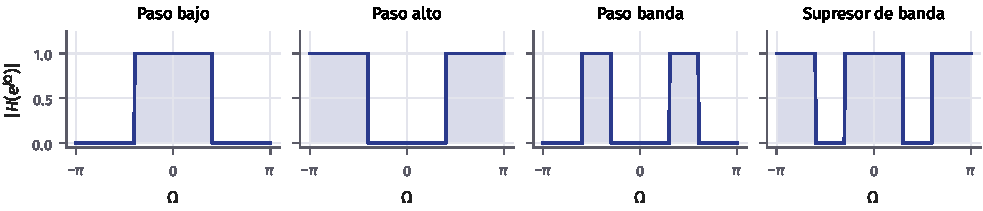
\includegraphics[width=\linewidth]{ideales}
  \caption{Los cuatro filtros ideales en discreto.}\label{fig:ideales}
\end{figure}

\begin{nota}[Erratas de versiones anteriores]
  En las transparencias antiguas el paso banda y el supresor ideales se escribían como $\omega_{c1}<\omega<\omega_{c2}$, sin valor absoluto, y el paso alto de la parte FIR como «$1$ si $\abs\omega<\omega_c$». Las definiciones correctas son las de arriba.
\end{nota}

Ningún filtro ideal se puede construir. La respuesta al impulso del paso bajo ideal es
\[
  h[n]=\frac1{2\pi}\int_{-\Omega_c}^{\Omega_c}\e^{j\Omega n}\dd\Omega=\frac{\sin(\Omega_cn)}{\pi n}
\]
(con $h[0]=\Omega_c/\pi$), que es distinta de cero para $n<0$, de modo que el sistema no es causal, y tiene duración infinita. En continuo ocurre lo mismo con $h(t)=\sin(\omega_ct)/(\pi t)$. Diseñar un filtro consiste en \emph{aproximar} el ideal con un sistema causal, estable y de orden finito, admitiendo una tolerancia.

\subsection{Especificaciones}

La tolerancia se expresa con una \emph{plantilla} (\cref{fig:especificaciones}). Para un paso bajo:
\begin{itemize}
  \item en la banda de paso, $0\le\omega\le\omega_p$, la atenuación no supera $\alpha_p$\,dB: $1/E\le\abs{H}\le1$ con $\alpha_p=20\log_{10}E$;
  \item en la banda de supresión, $\omega\ge\omega_s$, la atenuación es al menos $\alpha_s$\,dB: $\abs H\le1/A$ con $\alpha_s=20\log_{10}A$;
  \item en la banda de transición, $\omega_p<\omega<\omega_s$, no se impone nada.
\end{itemize}
La \emph{frecuencia de corte} $\omega_c$ es aquella en la que $\abs{H(j\omega_c)}=1/\sqrt2$, es decir, la atenuación es de 3\,dB. Dos cocientes resumen la dificultad del diseño: la \emph{selectividad} $k=\omega_p/\omega_s<1$, más exigente cuanto más se acerca a 1, y la \emph{discriminación}
\[
  k_1=\frac{\varepsilon}{\sqrt{A^2-1}},\qquad \varepsilon=\sqrt{E^2-1},
\]
más exigente cuanto más pequeña. En los filtros FIR es más habitual dar los rizados: $1-\delta_p\le\abs H\le1+\delta_p$ en la banda de paso y $\abs H\le\delta_s$ en la de supresión, con $\alpha_s=-20\log_{10}\delta_s$. Para los demás tipos de filtro hay un par de bordes por cada transición ($\omega_{p1},\omega_{p2},\omega_{s1},\omega_{s2}$ en un paso banda).

\begin{figure}[ht]
  \centering
  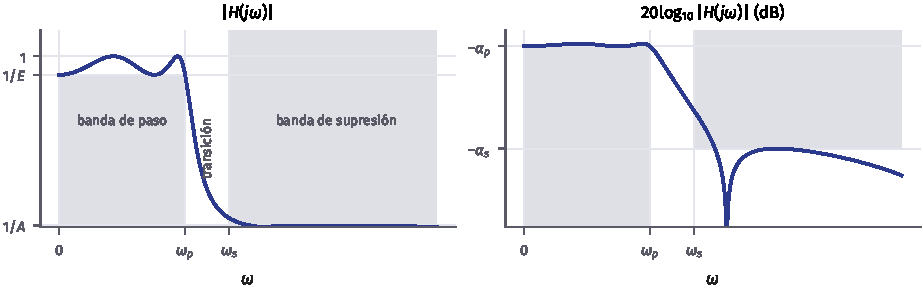
\includegraphics[width=0.9\linewidth]{especificaciones}
  \caption{Plantilla de un paso bajo en escala lineal y en decibelios, con un filtro elíptico que la cumple. Las zonas sombreadas están prohibidas.}\label{fig:especificaciones}
\end{figure}

\subsection{Fase y retardo de grupo}

Un sistema que no distorsiona solo escala y retrasa: $y[n]=K\,x[n-n_0]$, con $H(\e^{j\Omega})=K\e^{-j\Omega n_0}$. Su fase es \emph{lineal} en $\Omega$. En general se define el \emph{retardo de grupo}
\[
  \tau(\Omega)=-\frac{\dd\arg H(\e^{j\Omega})}{\dd\Omega}\quad\text{(muestras)},
\]
que mide cuánto se retrasa la envolvente de un paquete de frecuencias en torno a $\Omega$. Si $\tau$ es constante, todas las componentes se retrasan lo mismo y la forma de onda se conserva; si no, se produce \emph{distorsión de fase}. La \cref{fig:retardo} lo ilustra con una onda cuadrada: un IIR y un FIR con módulos parecidos dan salidas muy distintas, porque el IIR retrasa más los armónicos cercanos al corte. La distorsión de fase importa en transmisión de datos, en electrocardiografía o en audio de alta calidad; el oído es poco sensible a ella en régimen permanente, pero no en los transitorios.

\begin{figure}[ht]
  \centering
  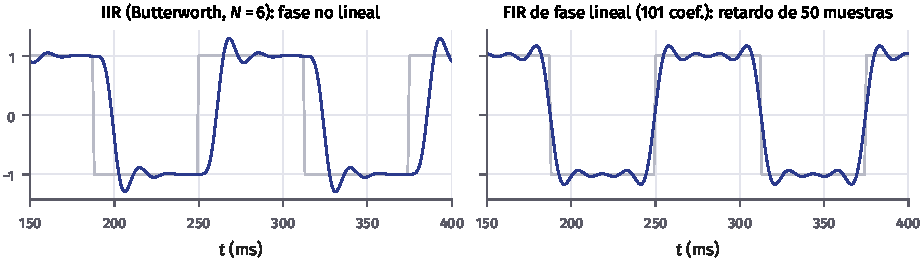
\includegraphics[width=0.95\linewidth]{retardo_grupo}
  \caption{Onda cuadrada de 8\,Hz ($f_s=1$\,kHz) filtrada con un Butterworth de orden 6 y con un FIR de fase lineal de 101 coeficientes, ambos con corte en 60\,Hz. La salida del FIR se ha adelantado 50 muestras para compararla.}\label{fig:retardo}
\end{figure}

\subsection{Polos, ceros y diseño a mano}

La respuesta en frecuencia de un sistema racional queda determinada por la posición de sus polos y ceros, que conocemos del Tema~1 (\cref{fig:pz-continuo}):
\begin{itemize}
  \item un \emph{polo real} en $-a$, $H(s)=a/(s+a)$, atenúa a partir de $\omega\approx a$ con una pendiente de $-20$\,dB/década, y cada polo adicional añade otros $-20$\,dB/década;
  \item un \emph{par de polos} $-\sigma\pm j\omega_a$ produce una resonancia cerca de $\omega_a$, tanto más aguda cuanto menor es $\sigma$. Con $\sigma=0$, $H(s)=\omega_n^2/(s^2+\omega_n^2)$ tiene los polos sobre el eje imaginario: es \emph{marginalmente estable}, su respuesta al impulso es una sinusoide que no se amortigua y no sirve como filtro;
  \item un \emph{par de ceros} en $\pm j\omega_n$ anula exactamente la frecuencia $\omega_n$. Sin polos, $\abs H$ crecería como $\omega^2$; con dos polos con parte real negativa el sistema es propio (tantos polos como ceros, condición para que sea realizable) y la ganancia vuelve a 1 lejos de $\omega_n$.
\end{itemize}

\begin{figure}[ht]
  \centering
  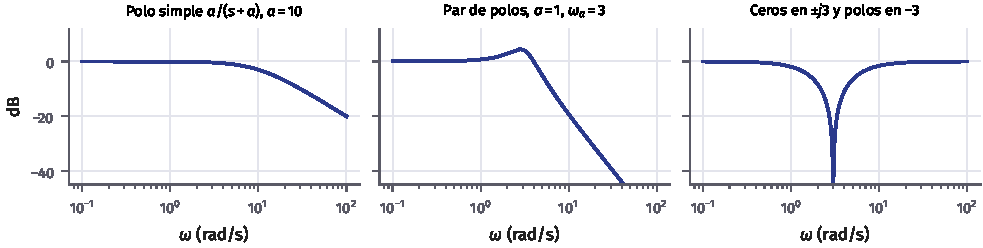
\includegraphics[width=\linewidth]{polos_ceros_continuo}
  \caption{Efecto de un polo real, de un par de polos complejos y de un par de ceros imaginarios compensado con dos polos.}\label{fig:pz-continuo}
\end{figure}

\begin{nota}[Erratas de versiones anteriores]
  Las transparencias antiguas decían que $\omega_n^2/(s^2+\omega_n^2)$ «es inestable para $\omega=\omega_n$»: el sistema es marginalmente estable (lo es o no para todas las frecuencias a la vez) y, en todo caso, queda fuera de los filtros que estudiamos, que son estables. También mezclaban $w_a$ y $\omega_a$ en la misma expresión.
\end{nota}

En discreto se razona igual con la circunferencia unidad en lugar del eje $j\omega$. Un \emph{filtro de muesca} que elimine $\Omega_0$ tiene ceros en $\e^{\pm j\Omega_0}$ y polos en el mismo ángulo con radio $r<1$:
\[
  H(z)=\frac{(1-\e^{j\Omega_0}z^{-1})(1-\e^{-j\Omega_0}z^{-1})}{(1-r\e^{j\Omega_0}z^{-1})(1-r\e^{-j\Omega_0}z^{-1})}
  =\frac{1-2\cos\Omega_0\,z^{-1}+z^{-2}}{1-2r\cos\Omega_0\,z^{-1}+r^2z^{-2}}.
\]
Lejos de $\Omega_0$ cada polo está casi a la misma distancia del punto $\e^{j\Omega}$ que su cero, y $\abs H\approx1$; la anchura de la muesca es aproximadamente $2(1-r)$\,rad (\cref{fig:notch}). Este diseño a mano funciona para filtros muy sencillos, pero no para filtros selectivos con especificaciones exigentes: para ellos hacen falta los métodos sistemáticos de las secciones siguientes.

\begin{figure}[ht]
  \centering
  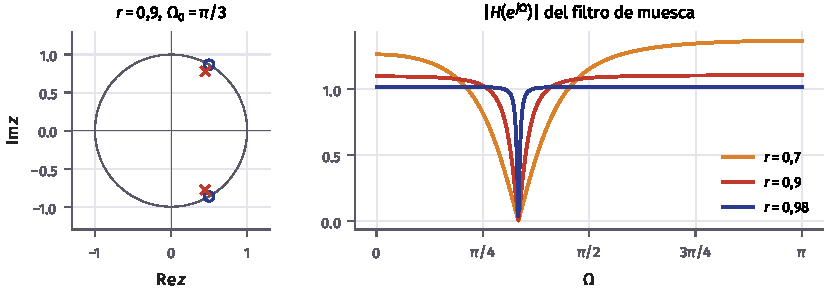
\includegraphics[width=0.85\linewidth]{notch_discreto}
  \caption{Filtro de muesca en $\Omega_0=\pi/3$: diagrama de polos y ceros y respuesta para tres radios.}\label{fig:notch}
\end{figure}

\subsection{Filtros FIR e IIR}

Un filtro discreto causal de orden finito tiene función de transferencia y ecuación en diferencias
\[
  H(z)=\frac{\sum_{k=0}^{M}b_kz^{-k}}{1+\sum_{k=1}^{N}a_kz^{-k}},\qquad
  y[n]=\sum_{k=0}^{M}b_k\,x[n-k]-\sum_{k=1}^{N}a_k\,y[n-k].
\]
Si algún $a_k\ne0$ hay realimentación y la respuesta al impulso es infinita: filtro \emph{IIR}. Si todos los $a_k$ son nulos, $h[n]=b_n$ tiene $M+1$ muestras: filtro \emph{FIR}. La \cref{tab:fir-iir} resume sus diferencias, que guían la elección.

\begin{table}[ht]
  \centering\small
  \caption{Comparación entre filtros IIR y FIR.}\label{tab:fir-iir}
  \begin{tabular}{@{}p{0.2\linewidth}p{0.36\linewidth}p{0.36\linewidth}@{}}
    \toprule
    & IIR & FIR\\\midrule
    Diseño & A partir de un filtro continuo & Directo en discreto (ventanas, optimización)\\
    Orden & Bajo & Alto: decenas o cientos de coeficientes\\
    Fase & No lineal & Puede ser exactamente lineal\\
    Estabilidad & Hay que comprobarla & Siempre estables\\
    Implementación & Sensible a la cuantificación; secciones de orden 2 & Robusta; admite FFT para órdenes altos\\\bottomrule
  \end{tabular}
\end{table}

\begin{flushright}\small\color{pdsgris}Ejercicios 1–3. \herramienta{server/T4\_Filtros\_Discretos\_PZMap.py}.\end{flushright}

% =====================================================================
\section{Filtros continuos}\label{sec:continuos}

\subsection{Aproximación del módulo}

Diseñamos un paso bajo continuo, el \emph{prototipo}, y obtendremos los demás tipos con transformaciones de frecuencia (\cref{sec:transformaciones}). Como $\abs{H(j\omega)}^2$ es una función par de $\omega$, se busca de la forma
\[
  \abs{H(j\omega)}^2=\frac{1}{1+P(\omega^2)},
\]
con $P$ pequeño en la banda de paso y grande en la de supresión. Cada familia de filtros corresponde a una elección de $P$. Conocido $\abs{H(j\omega)}^2=H(s)H(-s)\big|_{s=j\omega}$, se calculan las raíces de $H(s)H(-s)$, que aparecen en parejas simétricas respecto al eje imaginario, y se asignan a $H(s)$ las del semiplano izquierdo: el filtro resulta estable.

\begin{nota}[Erratas de versiones anteriores]
  Las transparencias antiguas escribían $\abs{H(j\omega)}=1/(1+P(\omega))$. Lo que se diseña es el cuadrado del módulo y $P$ depende de $\omega^2$; con la forma antigua no salen las fórmulas de Butterworth y Chebyshev que siguen.
\end{nota}

Los datos del diseño son $\omega_p$, $\omega_s$, $\alpha_p$ y $\alpha_s$, y de ellos se derivan
\[
  E=10^{\alpha_p/20},\quad A=10^{\alpha_s/20},\quad \varepsilon=\sqrt{E^2-1},\quad k=\frac{\omega_p}{\omega_s},\quad k_1=\frac{\varepsilon}{\sqrt{A^2-1}}.
\]
Usaremos como ejemplo común un paso bajo con $\alpha_p=1$\,dB hasta 1\,kHz y $\alpha_s=40$\,dB desde 5\,kHz: $\omega_p=2\pi\cdot1000$\,rad/s, $\omega_s=2\pi\cdot5000$\,rad/s, $E=1{,}122$, $A=100$, $\varepsilon=0{,}5088$, $k=0{,}2$ y $k_1=0{,}00509$.

\subsection{Butterworth}

\begin{definicion}{Filtro de Butterworth}{butterworth}
  \[
    \abs{H(j\omega)}^2=\frac{1}{1+(\omega/\omega_c)^{2N}}
  \]
\end{definicion}

Es \emph{máximamente plano}: las $2N-1$ primeras derivadas de $\abs H^2$ se anulan en $\omega=0$. Es monótono, vale $1/\sqrt2$ en $\omega_c$ sea cual sea el orden y cae $20N$\,dB/década. Las raíces de $1+(s/j\omega_c)^{2N}=0$ están sobre una circunferencia de radio $\omega_c$; las del semiplano izquierdo son los polos
\[
  p_k=\omega_c\,\e^{j\pi\frac{2k+N-1}{2N}},\qquad k=1,\dots,N,
\]
separados un ángulo $\pi/N$ (\cref{fig:butterworth}).

\begin{figure}[ht]
  \centering
  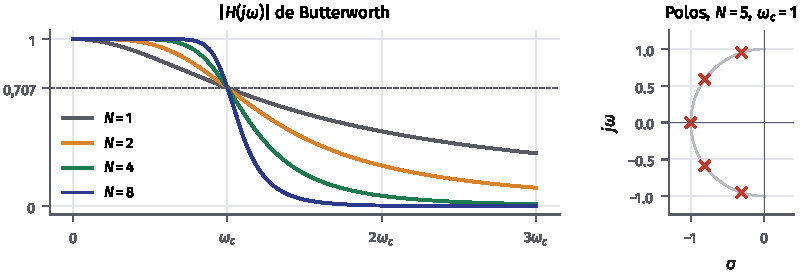
\includegraphics[width=0.9\linewidth]{butterworth_orden}
  \caption{Módulo del filtro de Butterworth para varios órdenes y polos para $N=5$.}\label{fig:butterworth}
\end{figure}

Para obtener el orden se imponen los dos bordes de la plantilla:
\[
  \frac{1}{1+(\omega_p/\omega_c)^{2N}}\ge\frac1{E^2}\ \Leftrightarrow\ \Big(\frac{\omega_p}{\omega_c}\Big)^{2N}\le E^2-1,\qquad
  \frac{1}{1+(\omega_s/\omega_c)^{2N}}\le\frac1{A^2}\ \Leftrightarrow\ \Big(\frac{\omega_s}{\omega_c}\Big)^{2N}\ge A^2-1.
\]
Dividiendo una entre otra se elimina $\omega_c$.

\begin{propiedad}{Orden y corte de un Butterworth}{orden-butter}
  \[
    N\ge\frac{\log_{10}\dfrac{A^2-1}{E^2-1}}{2\log_{10}\dfrac{\omega_s}{\omega_p}}=\frac{\log(1/k_1)}{\log(1/k)},\qquad
    \frac{\omega_p}{(E^2-1)^{1/2N}}\le\omega_c\le\frac{\omega_s}{(A^2-1)^{1/2N}}.
  \]
\end{propiedad}

Al redondear $N$ hacia arriba queda margen y $\omega_c$ se puede elegir en un intervalo: en el extremo izquierdo se cumple exactamente la banda de paso; en el derecho, la de supresión. \texttt{buttord} de Matlab y de \texttt{scipy.signal} devuelve el izquierdo.

\begin{ejemplo}{Butterworth}{butter}
  Con las especificaciones comunes, $E^2-1=0{,}2589$ y $A^2-1=9999$:
  \[
    N\ge\frac{\log_{10}(9999/0{,}2589)}{2\log_{10}5}=\frac{4{,}587}{1{,}398}=3{,}28\ \to\ N=4,
  \]
  \[
    \omega_c\in\Big[\frac{6283}{0{,}2589^{1/8}},\ \frac{31416}{9999^{1/8}}\Big]=[7439,\ 9935]\ \text{rad/s},
  \]
  es decir, $f_c$ entre 1184 y 1581\,Hz.
\end{ejemplo}

\begin{encodigo}
  Orden, corte y respuesta del Butterworth del ejemplo~\ref{ej:butter}.
  \codigo{butter_continuo}
\end{encodigo}

\subsection{Chebyshev}

Los \emph{polinomios de Chebyshev} se definen por
\[
  T_N(x)=\begin{cases}\cos(N\arccos x)&\abs x\le1\\\cosh(N\,\mathrm{arccosh}\,x)&\abs x>1\end{cases},\qquad
  T_0=1,\ T_1=x,\ T_{N+1}=2xT_N-T_{N-1}.
\]
En $[-1,1]$ oscilan entre $-1$ y $1$, con $N$ ceros; fuera crecen como $2^{N-1}x^N$, mucho más deprisa que $x^N$.

\begin{definicion}{Filtros de Chebyshev}{chebyshev}
  \[
    \text{Tipo I: }\abs{H(j\omega)}^2=\frac{1}{1+\varepsilon^2T_N^2(\omega/\omega_p)},\qquad
    \text{Tipo II: }\abs{H(j\omega)}^2=\frac{\varepsilon_2^2\,T_N^2(\omega_s/\omega)}{1+\varepsilon_2^2\,T_N^2(\omega_s/\omega)},\ \varepsilon_2^2=A^2-1.
  \]
\end{definicion}

El tipo~I tiene rizado entre $1$ y $1/E$ en la banda de paso (equirrizado) y cae monótonamente en la de supresión; sus polos están sobre una elipse. El tipo~II, o inverso, es plano en la banda de paso y tiene rizado en la de supresión, donde alcanza exactamente $1/A$ en sus máximos; tiene ceros sobre el eje $j\omega$. Para el tipo I, la condición en $\omega_s$ es $1+\varepsilon^2\cosh^2\big(N\,\mathrm{arccosh}(\omega_s/\omega_p)\big)\ge A^2$, que da

\begin{propiedad}{Orden de un Chebyshev}{orden-cheby}
  \[
    N\ge\frac{\mathrm{arccosh}(1/k_1)}{\mathrm{arccosh}(1/k)}=\frac{\mathrm{arccosh}\big(\sqrt{A^2-1}/\varepsilon\big)}{\mathrm{arccosh}(\omega_s/\omega_p)},
  \]
  la misma para los dos tipos.
\end{propiedad}

Con las especificaciones comunes, $1/k_1=196{,}5$ y $N\ge\mathrm{arccosh}(196{,}5)/\mathrm{arccosh}(5)=5{,}97/2{,}29=2{,}61$, de modo que $N=3$: uno menos que Butterworth. En Matlab y en \texttt{scipy.signal}, \texttt{cheby1(N,Rp,Wp)} recibe el rizado de la banda de paso y su borde, y \texttt{cheby2(N,Rs,Ws)} la atenuación de la banda de supresión y el suyo.

\begin{nota}[Erratas de versiones anteriores]
  En el resumen de órdenes de Matlab de las transparencias antiguas aparecía \texttt{cheby2(N,ap,wc,...)}; el segundo argumento de \texttt{cheby2} es la atenuación de la banda de supresión, \texttt{Rs}. La expresión del tipo II con $\cos^2(N\arccos1)$ en el denominador tampoco era correcta; la forma habitual es la de la definición~\ref{def:chebyshev}.
\end{nota}

\subsection{Elíptico}

El filtro \emph{elíptico} o de Cauer usa una función racional de Chebyshev $R_N$, construida con funciones elípticas de Jacobi:
\[
  \abs{H(j\omega)}^2=\frac{1}{1+\varepsilon^2R_N^2(\omega/\omega_p)}.
\]
Tiene rizado en las dos bandas y ceros en el eje $j\omega$, y es el filtro de \emph{menor orden} que cumple unas especificaciones dadas. El orden exacto es
\[
  N\ge\frac{K(k)\,K\big(\sqrt{1-k_1^2}\big)}{K(k_1)\,K\big(\sqrt{1-k^2}\big)},
\]
con $K$ la integral elíptica completa de primera especie. Una aproximación muy precisa es
\[
  k'=\sqrt{1-k^2},\quad \rho_0=\frac{1-\sqrt{k'}}{2(1+\sqrt{k'})},\quad \rho=\rho_0+2\rho_0^5+15\rho_0^9+150\rho_0^{13},\quad N\ge\frac{2\log_{10}(4/k_1)}{\log_{10}(1/\rho)}.
\]
Para las especificaciones comunes, $k=\omega_p/\omega_s=0{,}2$, $k'=0{,}9798$, $\rho=0{,}002551$ y $N\ge2{,}23$, así que $N=3$, el mismo orden que Chebyshev pero con más margen.

\begin{nota}[Erratas de versiones anteriores]
  El ejemplo elíptico antiguo escribía $k=\omega_s/\omega_p=1/5$: el valor $1/5$ es correcto, pero corresponde a $k=\omega_p/\omega_s$. Además, la llamada \texttt{ellip(N,as,ap,wp,...)} tenía los dos primeros parámetros intercambiados: es \texttt{ellip(N,Rp,Rs,Wp)}.
\end{nota}

\subsection{Comparación}

La \cref{fig:tipos-continuos} muestra las cuatro familias con el mismo orden, y la \cref{fig:polos-tipos} sus polos y ceros. Cuanto más selectivo es un filtro, menos lineal es su fase: Butterworth es el de fase más lineal y el elíptico el de menos. La \cref{fig:ejemplo-continuo} compara los diseños de orden mínimo para la plantilla común.

\begin{figure}[ht]
  \centering
  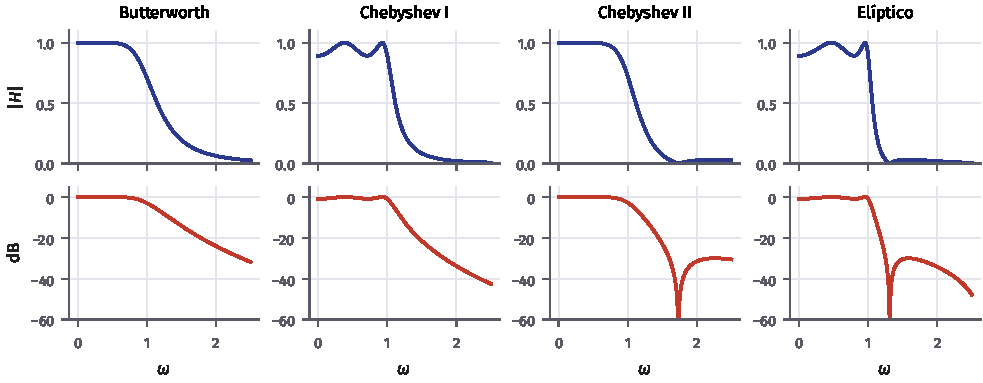
\includegraphics[width=\linewidth]{tipos_continuos}
  \caption{Butterworth, Chebyshev I y II y elíptico de orden 4, en escala lineal y en dB.}\label{fig:tipos-continuos}
\end{figure}

\begin{figure}[ht]
  \centering
  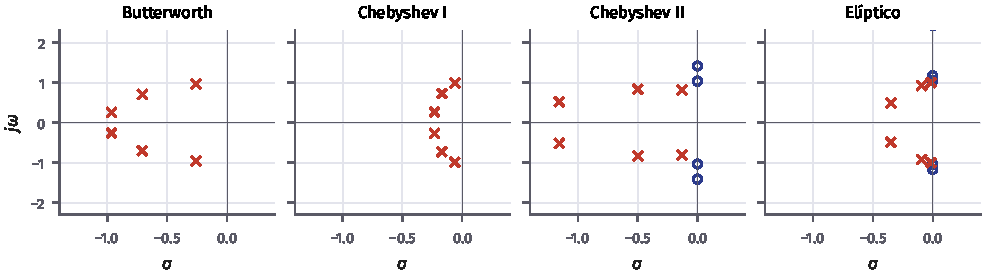
\includegraphics[width=\linewidth]{polos_tipos}
  \caption{Polos ($\times$) y ceros ($\circ$) de las cuatro familias para $N=6$.}\label{fig:polos-tipos}
\end{figure}

\begin{figure}[ht]
  \centering
  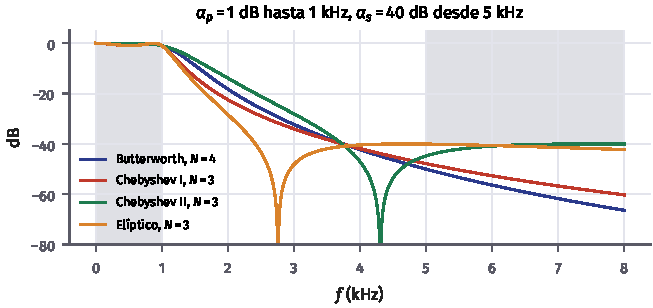
\includegraphics[width=0.7\linewidth]{ejemplo_continuo}
  \caption{Diseños de orden mínimo para la plantilla común.}\label{fig:ejemplo-continuo}
\end{figure}

\begin{encodigo}
  Orden mínimo de cada familia y llamadas de diseño, con el orden correcto de los argumentos.
  \codigo{orden_continuos}
\end{encodigo}

\subsection{Transformaciones de frecuencia}\label{sec:transformaciones}

Paso alto, paso banda y supresor se obtienen a partir de un prototipo paso bajo $H_{\text{LP}}(s)$ con $\omega_p=1$ mediante una sustitución $s=F(\hat s)$, donde $\hat s$ y $\hat\omega$ son la variable y la frecuencia del filtro de destino (\cref{tab:transformaciones}). Las transformaciones solo mueven las frecuencias: conservan los rizados y las atenuaciones.

\begin{table}[ht]
  \centering\small
  \renewcommand{\arraystretch}{1.8}
  \caption{Transformaciones de frecuencia desde un prototipo con $\omega_p=1$. En paso banda y supresor, $\hat\omega_0^2=\hat\omega_{p1}\hat\omega_{p2}$ y $B=\hat\omega_{p2}-\hat\omega_{p1}$.}\label{tab:transformaciones}
  \begin{tabular}{@{}llll@{}}
    \toprule
    Destino & Sustitución & Relación de frecuencias & Matlab / \texttt{scipy.signal}\\\midrule
    Paso bajo & $s=\hat s/\hat\omega_p$ & $\omega=\hat\omega/\hat\omega_p$ & \texttt{lp2lp}\\
    Paso alto & $s=\hat\omega_p/\hat s$ & $\omega=-\hat\omega_p/\hat\omega$ & \texttt{lp2hp}\\
    Paso banda & $s=\dfrac{\hat s^2+\hat\omega_0^2}{B\,\hat s}$ & $\omega=\dfrac{\hat\omega^2-\hat\omega_0^2}{B\,\hat\omega}$ & \texttt{lp2bp}\\
    Supresor & $s=\dfrac{B\,\hat s}{\hat s^2+\hat\omega_0^2}$ & $\omega=\dfrac{B\,\hat\omega}{\hat\omega_0^2-\hat\omega^2}$ & \texttt{lp2bs}\\\bottomrule
  \end{tabular}
\end{table}

El procedimiento es:
\begin{enumerate}
  \item llevar los bordes de supresión al prototipo con la relación de frecuencias y quedarse con el más exigente, $\omega_s=\min\abs{\omega(\hat\omega_s)}$;
  \item diseñar el prototipo con $\omega_p=1$, ese $\omega_s$, $\alpha_p$ y $\alpha_s$;
  \item sustituir: $H(\hat s)=H_{\text{LP}}(F(\hat s))$.
\end{enumerate}
El paso banda que resulta es geométricamente simétrico respecto a $\hat\omega_0$: dos frecuencias con la misma atenuación cumplen $\hat\omega_1\hat\omega_2=\hat\omega_0^2$. Si los bordes de supresión dados no lo son, uno de los dos se cumple con margen; por eso se toma el mínimo. El orden del paso banda y del supresor es el doble del del prototipo (\cref{fig:transformaciones}).

\begin{figure}[ht]
  \centering
  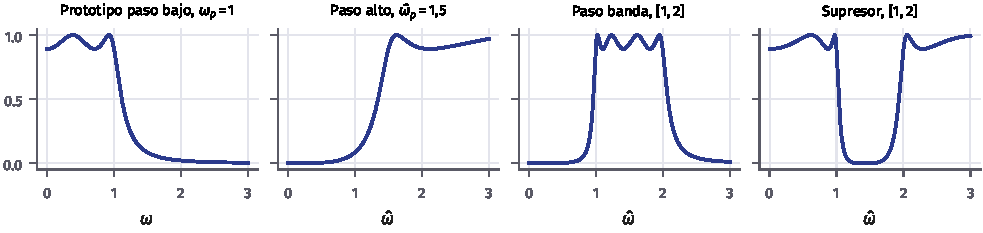
\includegraphics[width=\linewidth]{transformaciones}
  \caption{Un prototipo de Chebyshev I de orden 4 y los filtros que se obtienen con cada transformación.}\label{fig:transformaciones}
\end{figure}

\begin{ejemplo}{Paso alto de Butterworth}{pa-continuo}
  Banda de paso desde 4\,kHz con rizado de 0,1\,dB y atenuación mínima de 40\,dB por debajo de 1\,kHz. El prototipo tiene $\omega_p=1$ y $\omega_s=\hat\omega_p/\hat\omega_s=4$ (el signo de $\omega=-\hat\omega_p/\hat\omega$ no importa, porque $\abs H$ es par). Con $E^2-1=10^{0,01}-1=0{,}0233$,
  \[
    N\ge\frac{\log_{10}(9999/0{,}0233)}{2\log_{10}4}=4{,}68\ \to\ N=5,
  \]
  y el paso alto es $H(\hat s)=H_{\text{LP}}(2\pi\cdot4000/\hat s)$.
\end{ejemplo}

\begin{encodigo}
  El ejemplo~\ref{ej:pa-continuo} con el prototipo y \texttt{lp2hp}, y en un solo paso con \texttt{butter(N,wn,'high','s')}.
  \codigo{paso_alto_continuo}
\end{encodigo}

\begin{ejemplo}{Paso banda elíptico y supresor de Chebyshev II}{bp-continuo}
  \emph{Paso banda}: paso de 4 a 7\,kHz con 1\,dB; supresión por debajo de 3\,kHz y por encima de 8\,kHz con 22\,dB. Trabajando en kHz (el factor $2\pi$ se simplifica), $\hat\omega_0^2=28$ y $B=3$:
  \[
    \omega(3)=\frac{\abs{9-28}}{3\cdot3}=2{,}11,\qquad\omega(8)=\frac{64-28}{8\cdot3}=1{,}5,
  \]
  así que $\omega_s=1{,}5$ y un elíptico con $\alpha_p=1$, $\alpha_s=22$ necesita $N=3$ (orden 6).

  \emph{Supresor}: paso por debajo de 4 y por encima de 7\,kHz con 2\,dB; supresión entre 5 y 6\,kHz con 30\,dB. De nuevo $\hat\omega_0^2=28$, $B=3$:
  \[
    \omega(5)=\frac{5\cdot3}{28-25}=5,\qquad\omega(6)=\frac{6\cdot3}{36-28}=2{,}25,
  \]
  y $\omega_s=2{,}25$. El orden de Chebyshev es $N\ge\mathrm{arccosh}(41{,}3)/\mathrm{arccosh}(2{,}25)=3{,}02$, es decir, $N=4$. \texttt{cheb2ord} aplicada a las especificaciones originales da $N=3$, porque busca los bordes de paso que minimizan el orden: también es un diseño válido.
\end{ejemplo}

\begin{nota}[Erratas de versiones anteriores]
  Los ejemplos de paso banda y supresor antiguos decían «convertir el filtro paso bajo a paso alta» antes de usar \texttt{lp2bp} y \texttt{lp2bs}, hablaban de «atenuación superiora» (supresora) y de «rizo baso banda» (paso banda), y la frase «el filtro paso baja asociado al filtro paso baja» quería decir «el prototipo paso bajo asociado al filtro de destino». El ejemplo de paso banda antiguo llegaba a $\omega_s=1{,}4$ estrechando un borde de paso para hacer la plantilla simétrica; el resultado es más exigente que el necesario, pero válido.
\end{nota}

\begin{flushright}\small\color{pdsgris}Ejercicios 4–7. \herramienta{server/T4\_Filtros\_Continuos.py}.\end{flushright}

% =====================================================================
\section{Filtros IIR}\label{sec:iir}

Un filtro IIR se diseña casi siempre a partir de uno continuo: se obtiene $H_a(s)$ con los métodos de la \cref{sec:continuos} y se convierte en $H(z)$. La conversión debe llevar el eje $j\omega$ a la circunferencia unidad, para conservar la respuesta en frecuencia; el semiplano izquierdo al interior del círculo, para conservar la estabilidad; y dar un $H(z)$ racional.

\subsection{Invarianza al impulso}

La idea más directa es muestrear la respuesta al impulso: $h[n]=T\,h_a(nT)$ (el factor $T$ mantiene la ganancia en la banda de paso). Si $H_a$ tiene polos simples, por fracciones simples,
\[
  H_a(s)=\sum_k\frac{r_k}{s-p_k}\ \Rightarrow\ h_a(t)=\sum_kr_k\e^{p_kt}u(t)\ \Rightarrow\ H(z)=\sum_k\frac{T\,r_k}{1-\e^{p_kT}z^{-1}}.
\]
Cada polo $p_k$ se convierte en $\e^{p_kT}$, que está dentro del círculo si $\Re p_k<0$: la estabilidad se conserva. Pero, por el teorema del muestreo (Tema~2),
\[
  H(\e^{j\Omega})=\sum_{m=-\infty}^{\infty}H_a\Big(j\frac{\Omega-2\pi m}{T}\Big),
\]
y como ningún filtro continuo de orden finito está limitado en banda, siempre hay \emph{aliasing} (\cref{fig:invarianza}). Es tolerable si $H_a$ es despreciable por encima de $\pi/T$, lo que ocurre con paso bajo y paso banda; con paso alto y supresor de banda el método no sirve. Se usa sobre todo cuando interesa reproducir la forma de $h_a(t)$, por ejemplo al simular un sistema continuo.

\begin{figure}[ht]
  \centering
  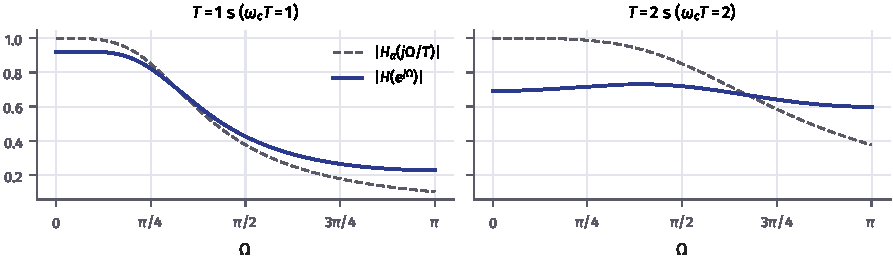
\includegraphics[width=0.9\linewidth]{invarianza}
  \caption{Invarianza al impulso de un Butterworth de orden 2 con $\omega_c=1$\,rad/s y dos periodos de muestreo. Con $T=2$\,s el aliasing deforma por completo la respuesta.}\label{fig:invarianza}
\end{figure}

\subsection{Transformada bilineal}

\begin{definicion}{Transformada bilineal}{bilineal}
  \[
    s=\frac2T\,\frac{1-z^{-1}}{1+z^{-1}}\qquad\Longleftrightarrow\qquad z=\frac{1+sT/2}{1-sT/2},\qquad H(z)=H_a(s)\Big|_{s=\frac2T\frac{1-z^{-1}}{1+z^{-1}}}.
  \]
\end{definicion}

Aparece al integrar numéricamente con la regla del trapecio: $y[n]=y[n-1]+\frac T2(x[n]+x[n-1])$ tiene función de transferencia $\frac T2\frac{1+z^{-1}}{1-z^{-1}}$, que aproxima al integrador $1/s$. Con $s=\sigma+j\omega$, $\abs z^2=\frac{(1+\sigma T/2)^2+(\omega T/2)^2}{(1-\sigma T/2)^2+(\omega T/2)^2}$, que es menor que 1 si y solo si $\sigma<0$: el semiplano izquierdo va al \emph{interior} del círculo y el eje $j\omega$ \emph{sobre} la circunferencia. En $z=\e^{j\Omega}$,
\[
  j\omega=\frac2T\,\frac{1-\e^{-j\Omega}}{1+\e^{-j\Omega}}=\frac2T\,\frac{\e^{j\Omega/2}-\e^{-j\Omega/2}}{\e^{j\Omega/2}+\e^{-j\Omega/2}}=j\,\frac2T\tan\frac\Omega2.
\]

\begin{propiedad}{Relación de frecuencias de la bilineal}{compresion}
  \[
    \omega=\frac2T\tan\frac\Omega2,\qquad \Omega=2\arctan\frac{\omega T}{2}.
  \]
  Todo el eje $\omega\in[0,\infty)$ se comprime en $\Omega\in[0,\pi)$, sin aliasing.
\end{propiedad}

La compresión deforma las frecuencias (\cref{fig:bilineal}), pero conserva los niveles: un rizado de 1\,dB del filtro continuo es un rizado de 1\,dB del discreto. Para que los bordes del discreto queden en $\Omega_p$ y $\Omega_s$, hay que \emph{predistorsionar}: el filtro continuo se diseña con bordes $\omega_p=\frac2T\tan\frac{\Omega_p}{2}$ y $\omega_s=\frac2T\tan\frac{\Omega_s}{2}$. Como $T$ aparece en la predistorsión y en la bilineal, se cancela y no tiene por qué ser el periodo de muestreo; lo habitual es tomar $T=2$, con lo que $\omega=\tan(\Omega/2)$ y $s=\frac{1-z^{-1}}{1+z^{-1}}$. Los ceros en el infinito de un paso bajo continuo van a $\Omega=\pi$, es decir, a $z=-1$.

\begin{figure}[ht]
  \centering
  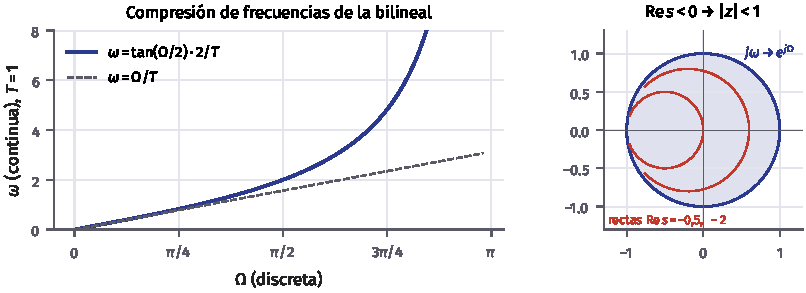
\includegraphics[width=0.9\linewidth]{bilineal}
  \caption{Relación de frecuencias de la bilineal ($T=1$) y transformación del semiplano izquierdo en el interior del círculo unidad.}\label{fig:bilineal}
\end{figure}

\begin{nota}[Erratas de versiones anteriores]
  Las transparencias antiguas decían que la bilineal lleva «el semiplano izquierdo al círculo unidad»: lo lleva al \emph{interior}; es el eje $j\omega$ el que va a la circunferencia. Usaban $\omega_d$ y $\omega_a$ para las frecuencias discreta y continua; aquí son $\Omega$ y $\omega$.
\end{nota}

\subsection{Procedimiento de diseño}

\begin{enumerate}
  \item Pasar los bordes a frecuencia discreta, $\Omega=2\pi f/f_s$. Las atenuaciones no cambian.
  \item Predistorsionar con $T=2$: $\omega=\tan(\Omega/2)$ en cada borde.
  \item Diseñar el filtro continuo: prototipo paso bajo y, si hace falta, transformación de frecuencias.
  \item Aplicar la bilineal, $H(z)=H_a\big(\frac{1-z^{-1}}{1+z^{-1}}\big)$; con \texttt{bilinear} se indica $f_s=1/T=0{,}5$.
  \item Comprobar la respuesta con \texttt{freqz}.
\end{enumerate}

\begin{ejemplo}{Paso bajo de Butterworth}{iir-pb}
  $f_s=200$\,kHz, banda de paso hasta 25\,kHz con rizado de 0,5\,dB y atenuación mínima de 15\,dB desde 55\,kHz. Los bordes discretos son $\Omega_p=2\pi\cdot25/200=0{,}25\pi$ y $\Omega_s=0{,}55\pi$, y predistorsionados $\omega_p=\tan(0{,}125\pi)=0{,}4142$ y $\omega_s=\tan(0{,}275\pi)=1{,}1708$. Con $E^2-1=0{,}1220$ y $A^2-1=30{,}62$,
  \[
    N\ge\frac{\log_{10}(30{,}62/0{,}1220)}{2\log_{10}(1{,}1708/0{,}4142)}=2{,}66\ \to\ N=3,\qquad \omega_c\in[0{,}588,\ 0{,}663].
  \]
  Con $\omega_c=0{,}588$ y la bilineal,
  \[
    H(z)=\frac{0{,}0662\,(1+z^{-1})^3}{1-0{,}9357z^{-1}+0{,}5672z^{-2}-0{,}1016z^{-3}},
  \]
  que atenúa 18\,dB a 55\,kHz (\cref{fig:iir-pb}).
\end{ejemplo}

\begin{figure}[ht]
  \centering
  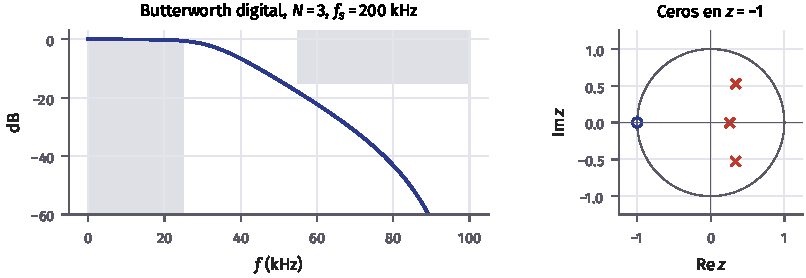
\includegraphics[width=0.9\linewidth]{iir_paso_bajo}
  \caption{Respuesta y polos y ceros del ejemplo~\ref{ej:iir-pb}.}\label{fig:iir-pb}
\end{figure}

\begin{encodigo}
  El ejemplo~\ref{ej:iir-pb} paso a paso (predistorsión, diseño continuo, bilineal) y con una sola llamada a \texttt{butter} con frecuencias discretas.
  \codigo{iir_bilineal}
\end{encodigo}

Si se omite \texttt{'s'} (o \texttt{analog=True}), las funciones de orden y diseño de Matlab y \texttt{scipy.signal} hacen la predistorsión y la bilineal internamente; las frecuencias se dan normalizadas a la de Nyquist, $\Omega/\pi\in[0,1]$, o en hercios con el argumento \texttt{fs} de \texttt{scipy}. El tipo se indica con \texttt{'high'} y \texttt{'stop'} en Matlab, y con \texttt{'highpass'}, \texttt{'bandpass'} y \texttt{'bandstop'} en Python.

\begin{nota}[Erratas de versiones anteriores]
  Una transparencia antigua decía que, con $T=2$, la orden \texttt{bilinear} se llama con tercer parámetro 0,5. Es correcto, pero la frase estaba incompleta («hacen de la orden bilineal se llamen»).
\end{nota}

\begin{ejemplo}{Paso alto de Chebyshev I y paso banda de Butterworth}{iir-otros}
  \emph{Paso alto}, $f_s=2$\,kHz: paso desde 700\,Hz con 1\,dB, supresión por debajo de 500\,Hz con 32\,dB. $\Omega_p=0{,}7\pi$ y $\Omega_s=0{,}5\pi$ dan $\hat\omega_p=\tan(0{,}35\pi)=1{,}9626$ y $\hat\omega_s=1$. En el prototipo, $\omega_s=\hat\omega_p/\hat\omega_s=1{,}9626$ y, con $\sqrt{A^2-1}/\varepsilon=78{,}2$,
  $N\ge\mathrm{arccosh}(78{,}2)/\mathrm{arccosh}(1{,}9626)=3{,}90$, es decir, $N=4$.

  \emph{Paso banda}: paso en $[0{,}45\pi,0{,}65\pi]$ con 1\,dB y supresión fuera de $[0{,}3\pi,0{,}75\pi]$ con 40\,dB. Predistorsionando, $\hat\omega_{p1}=0{,}8541$, $\hat\omega_{p2}=1{,}6319$, $\hat\omega_{s1}=0{,}5095$ y $\hat\omega_{s2}=2{,}4142$; $\hat\omega_0^2=1{,}3937$ y $B=0{,}7778$. Los bordes de supresión van a $2{,}86$ y $2{,}36$ en el prototipo, así que $\omega_s=2{,}36$ y $N\ge6{,}14$: $N=7$, un filtro de orden 14 (\cref{fig:iir-ejemplos}).
\end{ejemplo}

\begin{figure}[ht]
  \centering
  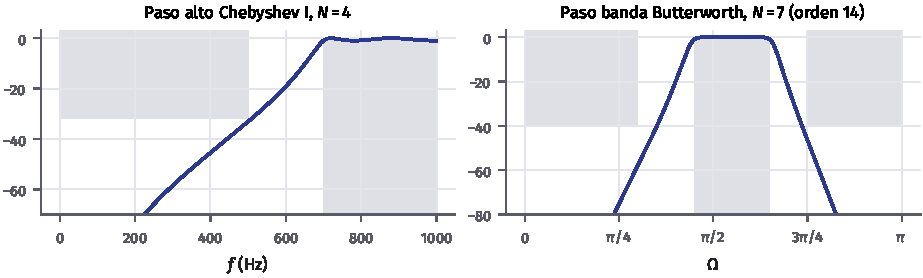
\includegraphics[width=0.9\linewidth]{iir_ejemplos}
  \caption{Filtros del ejemplo~\ref{ej:iir-otros}.}\label{fig:iir-ejemplos}
\end{figure}

\begin{encodigo}
  Diseño directo del paso banda del ejemplo~\ref{ej:iir-otros} en secciones de orden 2.
  \codigo{iir_paso_banda}
\end{encodigo}

\subsection{Transformaciones de frecuencia en discreto}

Alternativamente, se puede diseñar un paso bajo discreto con corte $\Omega_c$ y transformarlo sustituyendo $z^{-1}$ por un filtro paso todo de $\hat z^{-1}$, que lleva la circunferencia unidad sobre sí misma y el interior al interior (Constantinides, 1970). Las dos más sencillas son
\[
  \text{a paso bajo con corte }\hat\Omega_c:\ z^{-1}\to\frac{\hat z^{-1}-\alpha}{1-\alpha\hat z^{-1}},\quad\alpha=\frac{\sin\big((\Omega_c-\hat\Omega_c)/2\big)}{\sin\big((\Omega_c+\hat\Omega_c)/2\big)};
\]
\[
  \text{a paso alto con corte }\hat\Omega_c:\ z^{-1}\to-\frac{\hat z^{-1}+\alpha}{1+\alpha\hat z^{-1}},\quad\alpha=-\frac{\cos\big((\Omega_c+\hat\Omega_c)/2\big)}{\cos\big((\Omega_c-\hat\Omega_c)/2\big)}.
\]
Hay transformaciones de orden 2 a paso banda y supresor (Oppenheim y Schafer, capítulo 7). En Matlab están en \texttt{iirlp2hp}, \texttt{iirlp2bp} e \texttt{iirlp2bs}, con frecuencias normalizadas en $[0,1]$.

\begin{nota}[Erratas de versiones anteriores]
  La transparencia antigua daba para el paso alto $\lambda=-\cos\big((\omega_c-\hat\omega_c)/2\big)/\cos\big((\omega_c+\hat\omega_c)/2\big)$, con numerador y denominador intercambiados; en el supresor aparecía $\tan((\hat\omega_{c2}-\hat\omega_{c2})/2)$ en lugar de $\tan((\hat\omega_{c2}-\hat\omega_{c1})/2)$, y la función de Matlab \texttt{iirlp2sp} es \texttt{iirlp2bs}.
\end{nota}

\subsection{Implementación}

Un IIR de orden alto en forma directa (los coeficientes $a_k$ y $b_k$ del polinomio completo) es muy sensible al redondeo: las raíces de un polinomio de grado alto cambian mucho con pequeñas perturbaciones de sus coeficientes, y en los filtros selectivos los polos están muy juntos y cerca de la circunferencia. Se implementa como una cascada de \emph{secciones de orden 2} (\texttt{sos}), cada una con un par de polos y un par de ceros: \texttt{butter(..., output="sos")} y \texttt{sosfilt} en Python; \texttt{zp2sos} y \texttt{sosfilt} en Matlab. La \cref{tab:invarianza-bilineal} compara los dos métodos de conversión.

\begin{table}[ht]
  \centering\small
  \caption{Invarianza al impulso y transformada bilineal.}\label{tab:invarianza-bilineal}
  \begin{tabular}{@{}p{0.2\linewidth}p{0.36\linewidth}p{0.36\linewidth}@{}}
    \toprule
    & Invarianza al impulso & Bilineal\\\midrule
    Relación & $z=\e^{sT}$ para los polos & $s=\frac2T\frac{1-z^{-1}}{1+z^{-1}}$\\
    Frecuencias & Lineal, $\Omega=\omega T$ & Comprimidas, $\omega=\frac2T\tan\frac\Omega2$\\
    Aliasing & Sí & No\\
    Tipos & Paso bajo y paso banda & Todos\\
    Conserva & La forma de $h(t)$ & Los niveles de $\abs H$\\\bottomrule
  \end{tabular}
\end{table}

\begin{flushright}\small\color{pdsgris}Ejercicios 8–11. \herramienta{server/T4\_Filtros\_IIR\_Discretizacion.py}.\end{flushright}

% =====================================================================
\section{Filtros FIR}\label{sec:fir}

Un FIR de $N$ coeficientes (orden $N-1$) es
\[
  y[n]=\sum_{k=0}^{N-1}h[k]\,x[n-k],\qquad H(\e^{j\Omega})=\sum_{n=0}^{N-1}h[n]\,\e^{-j\Omega n}.
\]
Todos sus polos están en $z=0$, así que siempre es estable. No hay un filtro continuo del que partir, y se diseña directamente en discreto. Su mayor ventaja es que puede tener fase exactamente lineal.

\subsection{Fase lineal}

Si $h[n]$ es real y simétrica respecto a su centro $M=\frac{N-1}{2}$, $h[n]=h[N-1-n]$, los términos se agrupan por parejas:
\[
  h[n]\e^{-j\Omega n}+h[N-1-n]\e^{-j\Omega(N-1-n)}=\e^{-j\Omega M}\,h[n]\big(\e^{j\Omega(M-n)}+\e^{-j\Omega(M-n)}\big)=\e^{-j\Omega M}\,2h[n]\cos\big(\Omega(M-n)\big).
\]
Sumando todas las parejas (y el término central si $N$ es impar), $H(\e^{j\Omega})=\e^{-j\Omega M}A(\Omega)$ con $A(\Omega)$ real: la fase es lineal salvo saltos de $\pi$ donde $A$ cambia de signo, y el retardo de grupo vale $M=(N-1)/2$ muestras. Con antisimetría, $h[n]=-h[N-1-n]$, cada pareja da $2j\,h[n]\sin(\Omega(M-n))$ y $H=j\e^{-j\Omega M}A(\Omega)$: la fase es lineal con un desfase de $\pi/2$. Hay cuatro tipos (\cref{tab:tipos-fir}).

\begin{table}[ht]
  \centering\small
  \renewcommand{\arraystretch}{1.5}
  \caption{Los cuatro tipos de FIR de fase lineal, con $M=(N-1)/2$.}\label{tab:tipos-fir}
  \begin{tabular}{@{}lllll@{}}
    \toprule
    Tipo & Simetría & $N$ & $A(\Omega)$ & Ceros forzados\\\midrule
    I & par & impar & $h[M]+\sum_{n=0}^{M-1}2h[n]\cos(\Omega(M-n))$ & ninguno\\
    II & par & par & $\sum_{n=0}^{N/2-1}2h[n]\cos(\Omega(M-n))$ & $z=-1$\\
    III & impar & impar & $\sum_{n=0}^{M-1}2h[n]\sin(\Omega(M-n))$, con $h[M]=0$ & $z=1$ y $z=-1$\\
    IV & impar & par & $\sum_{n=0}^{N/2-1}2h[n]\sin(\Omega(M-n))$ & $z=1$\\\bottomrule
  \end{tabular}
\end{table}

Los ceros forzados se ven en $A(\Omega)$: en el tipo II, en $\Omega=\pi$ todos los cosenos $\cos(\pi(M-n))$ tienen argumento múltiplo impar de $\pi/2$ y se anulan; en los tipos III y IV los senos se anulan en $\Omega=0$, y en el III también en $\Omega=\pi$. Por eso el tipo II no puede ser paso alto ni supresor, el III solo puede ser paso banda, y el IV sirve para paso alto, derivadores y transformadores de Hilbert. El tipo I sirve para todo.

En el dominio $z$, la simetría equivale a $H(z)=\pm z^{-(N-1)}H(z^{-1})$: si $z_0$ es un cero, $1/z_0$ también lo es, y como $h$ es real, también $z_0^*$ y $1/z_0^*$. Los ceros aparecen en cuartetos, o en parejas recíprocas sobre el eje real, o en parejas conjugadas sobre la circunferencia (\cref{fig:tipos-fir}).

\begin{figure}[ht]
  \centering
  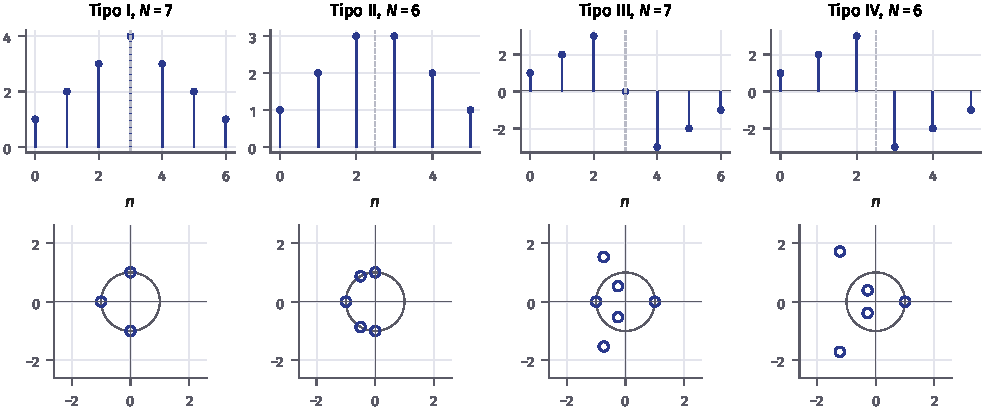
\includegraphics[width=0.95\linewidth]{tipos_fase_lineal}
  \caption{Un ejemplo de cada tipo y sus ceros. Obsérvense los ceros en $z=-1$ (tipos II y III) y en $z=1$ (tipos III y IV).}\label{fig:tipos-fir}
\end{figure}

\begin{nota}[Erratas de versiones anteriores]
  En la transparencia antigua de los ceros, los tipos aparecían con la paridad de $N$ cambiada («Tipo 1 ($N$ par)») y con números de ceros en $\pm1$ que no correspondían; la tabla resumen tenía el mismo problema. Lo correcto es la \cref{tab:tipos-fir}: en $z=-1$ hay un número impar de ceros en los tipos II y III, y en $z=1$ en los tipos III y IV. La nota a pie que decía que el desfase es $-\omega N/2$ se refiere a un filtro de $N+1$ coeficientes.
\end{nota}

\subsection{Método de las ventanas}

Se parte de la respuesta al impulso del filtro ideal con fase cero, $h_d[n]=\frac{1}{2\pi}\int_{-\pi}^{\pi}H_d(\e^{j\Omega})\e^{j\Omega n}\dd\Omega$ (\cref{tab:ideales}). Como $h_d$ es infinita y no causal:
\begin{enumerate}
  \item se trunca a $\abs n\le L$ ponderándola con una ventana $w[n]$: $h_w[n]=h_d[n]\,w[n]$, $N=2L+1$ coeficientes;
  \item se retrasa $L$ muestras: $h[n]=h_w[n-L]$, $0\le n\le 2L$ (\cref{fig:metodo-ventana}).
\end{enumerate}
$h_d$ y $w$ son pares, de modo que $h$ es simétrica, de tipo I, con $H(\e^{j\Omega})=\e^{-j\Omega L}H_w(\e^{j\Omega})$. Por el teorema de la modulación,
\[
  H_w(\e^{j\Omega})=\frac{1}{2\pi}\int_{-\pi}^{\pi}H_d(\e^{j\theta})\,W\big(\e^{j(\Omega-\theta)}\big)\dd\theta:
\]
el filtro ideal suavizado por la transformada de la ventana, igual que en el análisis espectral del Tema~3.

\begin{table}[ht]
  \centering\small
  \renewcommand{\arraystretch}{1.7}
  \caption{Respuestas al impulso de los filtros ideales con fase cero.}\label{tab:ideales}
  \begin{tabular}{@{}lll@{}}
    \toprule
    Filtro & $h_d[0]$ & $h_d[n]$, $n\ne0$\\\midrule
    Paso bajo ($\Omega_c$) & $\Omega_c/\pi$ & $\dfrac{\sin(\Omega_cn)}{\pi n}$\\
    Paso alto ($\Omega_c$) & $1-\Omega_c/\pi$ & $-\dfrac{\sin(\Omega_cn)}{\pi n}$\\
    Paso banda ($\Omega_1,\Omega_2$) & $(\Omega_2-\Omega_1)/\pi$ & $\dfrac{\sin(\Omega_2n)-\sin(\Omega_1n)}{\pi n}$\\
    Supresor ($\Omega_1,\Omega_2$) & $1-(\Omega_2-\Omega_1)/\pi$ & $-\dfrac{\sin(\Omega_2n)-\sin(\Omega_1n)}{\pi n}$\\
    Multibanda ($A_k$ en $[\Omega_{k-1},\Omega_k]$) & $\sum_kA_k\dfrac{\Omega_k-\Omega_{k-1}}{\pi}$ & $\sum_k(A_k-A_{k+1})\dfrac{\sin(\Omega_kn)}{\pi n}$, con $A_{M+1}=0$\\\bottomrule
  \end{tabular}
\end{table}

\begin{figure}[ht]
  \centering
  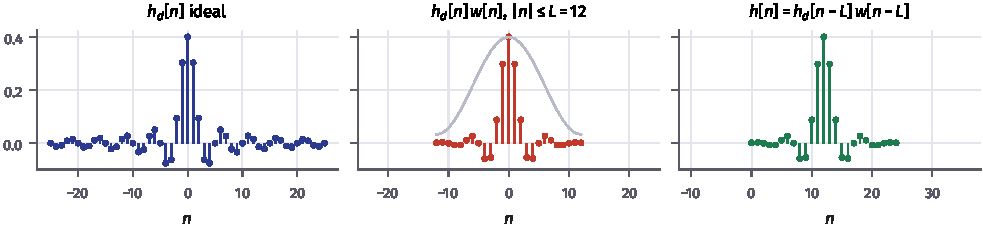
\includegraphics[width=\linewidth]{fir_ventana_metodo}
  \caption{Método de las ventanas: respuesta ideal, truncada y ponderada (Hamming, $L=12$), y retrasada.}\label{fig:metodo-ventana}
\end{figure}

\begin{nota}[Erratas de versiones anteriores]
  La expresión antigua del filtro multibanda ponderaba los senos con $A_k-A_{k-1}$; como $H=\sum_kA_k(H_{\text{PB},\Omega_k}-H_{\text{PB},\Omega_{k-1}})$, el coeficiente de $\sin(\Omega_kn)$ es $A_k-A_{k+1}$. En la diapositiva del procedimiento FIR, la ecuación $y[n]=\sum x[n-k]$ había perdido los coeficientes $b_k$, y se hablaba de «un FIR de orden $N+1$» con $N+1$ coeficientes (es de orden $N$).
\end{nota}

\subsection{Fenómeno de Gibbs y ventanas fijas}

Con la ventana rectangular (truncamiento simple), el lóbulo principal de $W$, de anchura $4\pi/(2L+1)$, fija la anchura de la transición, que se estrecha al crecer $L$. Los lóbulos secundarios fijan el rizado, y como su área relativa no depende de $L$, el rizado tampoco: alrededor de un 9\,\% de sobreoscilación junto al borde y un primer lóbulo en la banda de supresión hacia $-21$\,dB (\cref{fig:gibbs}). Es el \emph{fenómeno de Gibbs}. Para reducir el rizado hay que usar ventanas que vayan suavemente a cero en los extremos (\cref{fig:ventanas-fir}). Para $-L\le n\le L$:
\[
  w_{\text{Hann}}=\tfrac12+\tfrac12\cos\tfrac{2\pi n}{2L+1},\quad
  w_{\text{Hamming}}=0{,}54+0{,}46\cos\tfrac{2\pi n}{2L+1},
\]
\[
  w_{\text{Blackman}}=0{,}42+0{,}5\cos\tfrac{2\pi n}{2L+1}+0{,}08\cos\tfrac{4\pi n}{2L+1}.
\]

\begin{figure}[ht]
  \centering
  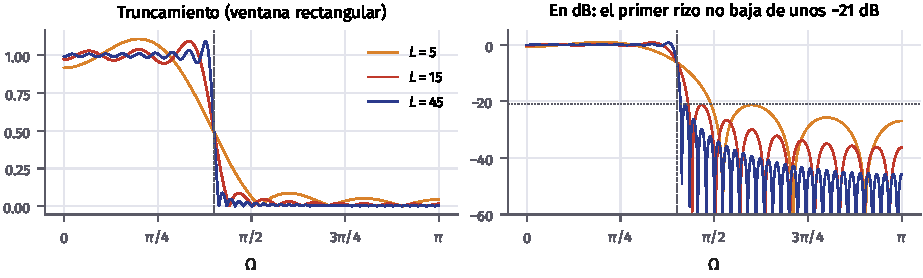
\includegraphics[width=0.9\linewidth]{gibbs}
  \caption{Truncamiento de un paso bajo ideal con $\Omega_c=0{,}4\pi$: la transición se estrecha al crecer $L$, pero el rizado no baja.}\label{fig:gibbs}
\end{figure}

\begin{figure}[ht]
  \centering
  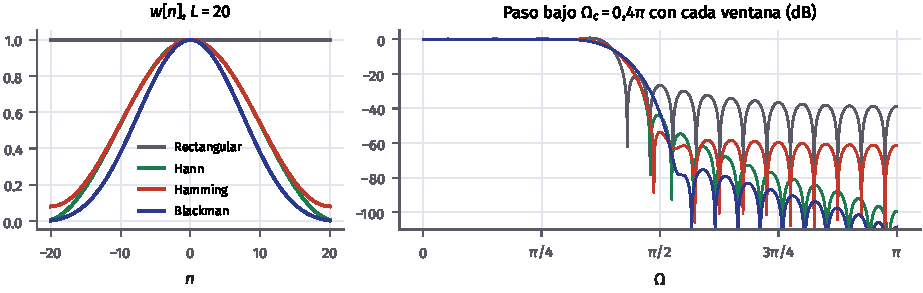
\includegraphics[width=0.9\linewidth]{ventanas_fir}
  \caption{Ventanas fijas con $L=20$ y el paso bajo que da cada una.}\label{fig:ventanas-fir}
\end{figure}

\begin{table}[ht]
  \centering\small
  \caption{Ventanas fijas para diseño de filtros (valores de Mitra). La atenuación mínima es la del filtro, no la del lóbulo secundario de la ventana.}\label{tab:ventanas-fir}
  \begin{tabular}{@{}lcccc@{}}
    \toprule
    Ventana & Lóbulo principal & Lóbulo secundario & Atenuación mínima $\alpha_s$ & Transición $\Delta\Omega$\\\midrule
    Rectangular & $4\pi/(2L+1)$ & $-13{,}3$\,dB & 20,9\,dB & $0{,}92\pi/L$\\
    Hann & $8\pi/(2L+1)$ & $-31{,}5$\,dB & 43,9\,dB & $3{,}11\pi/L$\\
    Hamming & $8\pi/(2L+1)$ & $-42{,}7$\,dB & 54,5\,dB & $3{,}32\pi/L$\\
    Blackman & $12\pi/(2L+1)$ & $-58{,}1$\,dB & 75,3\,dB & $5{,}56\pi/L$\\\bottomrule
  \end{tabular}
\end{table}

Con una ventana fija el rizado es el mismo en las dos bandas, $\delta_p\approx\delta_s$, y lo determina la ventana. El diseño se reduce a:
\begin{enumerate}
  \item corte en el centro de la transición, $\Omega_c=(\Omega_p+\Omega_s)/2$, donde $\abs H\approx0{,}5$;
  \item la ventana más sencilla con atenuación mínima mayor que $\alpha_s$;
  \item el menor $L$ cuya transición sea menor que $\Delta\Omega=\Omega_s-\Omega_p$.
\end{enumerate}

\begin{ejemplo}{Paso bajo con ventana fija}{fir-hann}
  $\Omega_p=0{,}3\pi$, $\Omega_s=0{,}5\pi$, $\alpha_s=40$\,dB. $\Omega_c=0{,}4\pi$ y $\Delta\Omega=0{,}2\pi$. Sirven Hann, Hamming y Blackman; con Hann, $L\ge3{,}11\pi/0{,}2\pi=15{,}6$, así que $L=16$ y $N=33$ coeficientes; Hamming pediría $L=17$ y Blackman $L=28$. La atenuación conseguida es de 44\,dB, con un retardo de 16 muestras.
\end{ejemplo}

\begin{nota}[Erratas de versiones anteriores]
  El ejemplo antiguo decía «filtros posibles son Hann, Hamming y Hamming»: el tercero es Blackman. En la fórmula de la ventana de Dolph–Chebyshev aparecía $T_{2N}$ (es $T_{2L}$), y en la definición de $T_l$ las dos ramas tenían la condición $\abs x<1$ (la segunda es $\abs x>1$).
\end{nota}

\begin{encodigo}
  El ejemplo~\ref{ej:fir-hann} construyendo $h[n]$ a mano y con \texttt{firwin}/\texttt{fir1}.
  \codigo{fir_ventana}
\end{encodigo}

\subsection{Ventana de Kaiser}

Las ventanas fijas no permiten elegir el rizado. La ventana de Kaiser tiene un parámetro $\beta$ que ajusta el compromiso entre rizado y anchura de transición (\cref{fig:kaiser}):
\[
  w[n]=\frac{I_0\big(\beta\sqrt{1-(n/L)^2}\big)}{I_0(\beta)},\quad\abs n\le L,\qquad I_0(u)=1+\sum_{r=1}^{\infty}\Big(\frac{(u/2)^r}{r!}\Big)^2,
\]
donde $I_0$ es la función de Bessel modificada de orden cero. Kaiser obtuvo fórmulas empíricas para $\beta$ y $L$:

\begin{propiedad}{Diseño con ventana de Kaiser}{kaiser}
  \[
    \beta=\begin{cases}0{,}1102\,(\alpha_s-8{,}7)&\alpha_s>50\\0{,}5842\,(\alpha_s-21)^{0{,}4}+0{,}07886\,(\alpha_s-21)&21\le\alpha_s\le50\\0&\alpha_s<21\end{cases},\qquad
    2L\ge\frac{\alpha_s-8}{2{,}285\,\Delta\Omega}.
  \]
\end{propiedad}

\begin{figure}[ht]
  \centering
  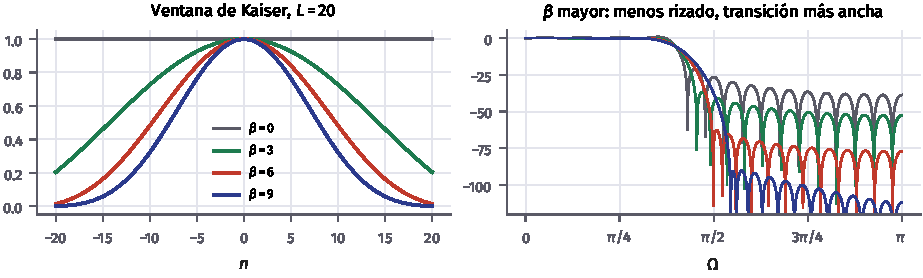
\includegraphics[width=0.9\linewidth]{kaiser}
  \caption{Ventana de Kaiser con $L=20$ para varios valores de $\beta$, y el paso bajo correspondiente.}\label{fig:kaiser}
\end{figure}

Para el ejemplo~\ref{ej:fir-hann}, $\beta=0{,}5842\cdot19^{0,4}+0{,}07886\cdot19=3{,}395$ y $2L\ge32/(2{,}285\cdot0{,}2\pi)=22{,}3$, de modo que $L=12$: 25 coeficientes en lugar de 33, con 41,7\,dB de atenuación (\cref{fig:ejemplo-fir}). Si se dan los rizados, $\alpha_s=-20\log_{10}\min(\delta_p,\delta_s)$, porque la ventana produce el mismo en las dos bandas. Otra ventana ajustable es la de \emph{Dolph–Chebyshev} (\texttt{chebwin}), que pone todos los lóbulos secundarios a la misma altura; para ella $2L\approx(2{,}056\alpha_s-16{,}4)/(2{,}285\Delta\Omega)$.

\begin{figure}[ht]
  \centering
  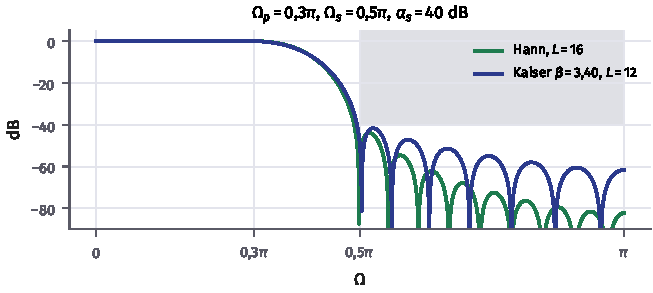
\includegraphics[width=0.65\linewidth]{ejemplo_fir}
  \caption{El paso bajo del ejemplo~\ref{ej:fir-hann} con Hann ($L=16$) y con Kaiser ($L=12$).}\label{fig:ejemplo-fir}
\end{figure}

\begin{nota}[Erratas de versiones anteriores]
  Las transparencias antiguas daban $0{,}5482$ en lugar de $0{,}5842$ en la fórmula de $\beta$, con lo que el ejemplo obtenía $\beta=3{,}278$ en lugar de $3{,}395$, y el intervalo intermedio aparecía como $50\le\alpha_s\le21$. El coeficiente del primer tramo es $0{,}1102$, no $0{,}11102$.
\end{nota}

\begin{encodigo}
  Paso alto con $\Omega_s=0{,}4\pi$, $\Omega_p=0{,}55\pi$ y $\delta=0{,}01$ con \texttt{kaiserord}, y el mismo filtro con Parks–McClellan. El paso alto debe ser de tipo I: si \texttt{kaiserord} propone un número par de coeficientes, se añade uno.
  \codigo{fir_kaiser}
\end{encodigo}

\subsection{Parks–McClellan y muestreo en frecuencia}

El método de Parks–McClellan busca el FIR de fase lineal que minimiza el \emph{error máximo} ponderado entre $A(\Omega)$ y la respuesta ideal en las bandas especificadas. El teorema de alternancia asegura que la solución es \emph{equirrizada}: el error alcanza su máximo con signos alternos en al menos $M+2$ frecuencias, y el algoritmo de Remez las encuentra. Con el mismo número de coeficientes, el rizado es menor que con cualquier ventana (\cref{fig:equirrizado}), y se pueden pedir rizados distintos en cada banda. El orden se estima con la fórmula de Kaiser
\[
  N-1\approx\frac{-20\log_{10}\sqrt{\delta_p\delta_s}-13}{14{,}6\,\Delta\Omega/2\pi}.
\]
Se usa con \texttt{firpm} en Matlab y \texttt{remez} en \texttt{scipy.signal}.

\begin{figure}[ht]
  \centering
  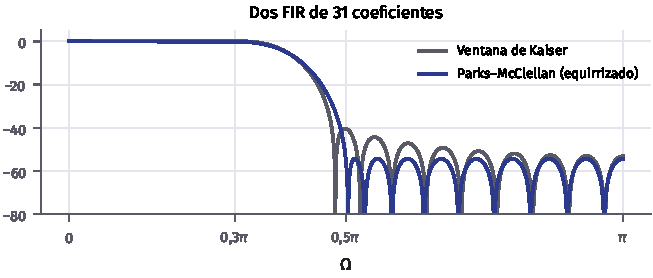
\includegraphics[width=0.65\linewidth]{equirrizado}
  \caption{FIR de 31 coeficientes con Kaiser y con Parks–McClellan para las mismas bandas.}\label{fig:equirrizado}
\end{figure}

En el \emph{muestreo en frecuencia} se fija la respuesta deseada en $N$ frecuencias $\Omega_k=2\pi k/N$ y se obtiene $h[n]$ con la IDFT, imponiendo la simetría de fase lineal. Entre las muestras, la respuesta interpola con rizado; se mejora dejando muestras de valor intermedio en la transición o aplicando una ventana a $h[n]$. \texttt{fir2} (Matlab) y \texttt{firwin2} (\texttt{scipy.signal}) hacen esto a partir de una respuesta definida a tramos, lo que permite filtros multibanda arbitrarios (\cref{fig:multibanda}).

\begin{figure}[ht]
  \centering
  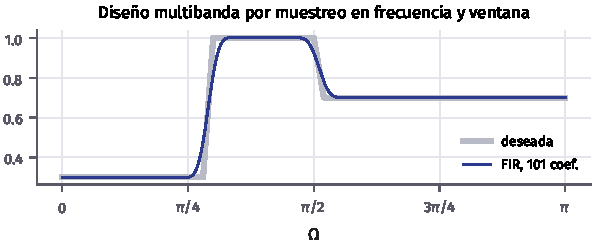
\includegraphics[width=0.6\linewidth]{multibanda}
  \caption{FIR multibanda de 101 coeficientes con \texttt{firwin2} y ventana de Hamming.}\label{fig:multibanda}
\end{figure}

\subsection{Coste y retardo}

Un FIR de $N$ coeficientes cuesta $N$ productos por muestra (la mitad aprovechando la simetría) y retrasa $(N-1)/2$ muestras. En audio a 44,1--48\,kHz son habituales 50--200 coeficientes en filtros básicos, 100--500 en filtros de cruce de altavoces, 500--2000 en cancelación de eco y hasta varios miles en procesado de alta calidad, con retardos de unos pocos a decenas de milisegundos. Para órdenes altos se filtra por bloques con la FFT (solapamiento y suma, Tema~3). En aplicaciones en tiempo real el retardo limita el orden; un IIR, o un FIR de fase mínima (\cref{sec:especiales}), retrasan mucho menos.

\begin{flushright}\small\color{pdsgris}Ejercicios 12–15. \herramienta{server/T4\_01\_FIR\_Ventana\_Fija.py} y \texttt{T4\_02\_FIR\_Kaiser.py}.\end{flushright}

% =====================================================================
\section{Filtros especiales}\label{sec:especiales}

\subsection{Fase cero}

Un filtro de fase cero tiene $H(\e^{j\Omega})$ real y no negativa, lo que exige $h[n]=h[-n]$: no es causal. Dado cualquier $F(z)$, $H(z)=F(z)F(z^{-1})$ es de fase cero, porque $H(\e^{j\Omega})=F(\e^{j\Omega})F^*(\e^{j\Omega})=\abs{F(\e^{j\Omega})}^2$ si $f$ es real. Sus polos y ceros aparecen en parejas recíprocas, así que $H$ no es causal y estable a la vez; pero si la señal está \emph{grabada} se puede aplicar en dos pasos: se filtra $x$ con $F$, se invierte la salida en el tiempo, se vuelve a filtrar y se invierte otra vez. Como invertir en el tiempo una señal real conjuga su DTFT,
\[
  Y=\big(F\,(F\,X)^*\big)^*=F^*F\,X=\abs F^2X.
\]
La atenuación en dB se duplica y la fase es nula (\cref{fig:fase-cero}). Es lo que hace \texttt{filtfilt} en Matlab y en \texttt{scipy.signal}, que además cuida los transitorios de los extremos.

\begin{figure}[ht]
  \centering
  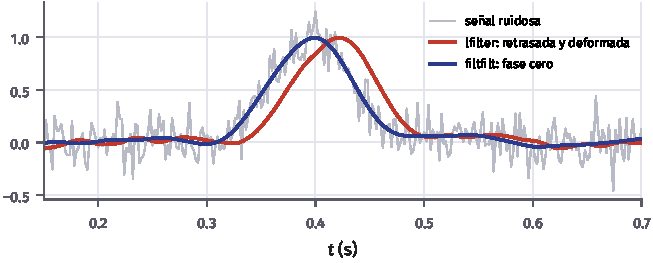
\includegraphics[width=0.65\linewidth]{fase_cero}
  \caption{Un pulso con ruido filtrado con un Butterworth de orden 3 hacia delante (\texttt{lfilter}) y con fase cero (\texttt{filtfilt}).}\label{fig:fase-cero}
\end{figure}

\begin{encodigo}
  Filtrado normal y de fase cero; se compara la posición del máximo.
  \codigo{fase_cero}
\end{encodigo}

\subsection{Fase mínima, máxima y mixta}

Reflejar un cero respecto a la circunferencia unidad, de $z_0$ a $1/z_0^*$, no cambia el módulo de la respuesta salvo una constante:
\[
  \abs{1-z_0\e^{-j\Omega}}=\abs{z_0}\,\Big|1-\frac{1}{z_0^*}\e^{-j\Omega}\Big|.
\]
Hay por tanto muchos sistemas con el mismo $\abs H$ y distinta fase. Un sistema causal y estable es de \emph{fase mínima} si todos sus ceros están dentro del círculo, de \emph{fase máxima} si están todos fuera y de \emph{fase mixta} en otro caso (\cref{fig:fase-minima}). El de fase mínima tiene el menor retardo de grupo y la menor variación de fase de todos los que comparten módulo, concentra la energía de $h[n]$ al principio, y es el único cuya inversa $1/H(z)$ también es causal y estable, lo que importa para deshacer el efecto de un canal.

\begin{figure}[ht]
  \centering
  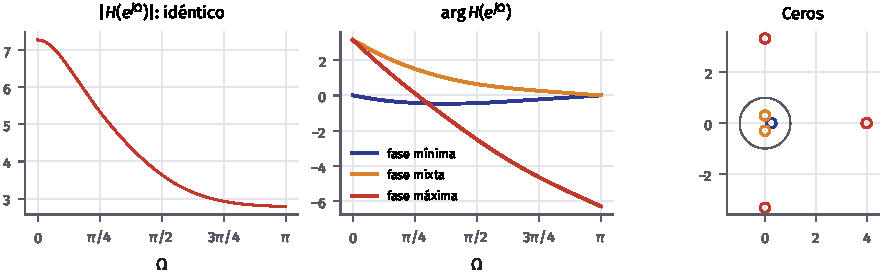
\includegraphics[width=0.95\linewidth]{fase_minima}
  \caption{Tres sistemas con los mismos polos y el mismo módulo y ceros reflejados: fase mínima, mixta y máxima.}\label{fig:fase-minima}
\end{figure}

\begin{nota}[Erratas de versiones anteriores]
  Las transparencias antiguas definían $H_{\text{MAX}}$ como un sistema «con todos sus ceros simétricos respecto al círculo unidad y el caso anterior»; quiere decir con los ceros de $H_{\text{MIN}}$ reflejados, todos fuera del círculo. La variación de fase adicional del de fase máxima está entre 0 y $N\pi$ en $[0,\pi]$, con $N$ el número de ceros reflejados.
\end{nota}

\subsection{Filtros paso todo}

Un filtro \emph{paso todo} tiene $\abs{H(\e^{j\Omega})}=1$ para toda $\Omega$. Con coeficientes reales y causal, tiene la forma
\[
  H_{\text{PT}}(z)=\frac{a_M+a_{M-1}z^{-1}+\dots+z^{-M}}{1+a_1z^{-1}+\dots+a_Mz^{-M}}=\frac{z^{-M}D(z^{-1})}{D(z)},
\]
con el numerador igual al denominador con los coeficientes en orden inverso. En la circunferencia, $\abs{\e^{-j\Omega M}D(\e^{-j\Omega})}=\abs{D^*(\e^{j\Omega})}=\abs{D(\e^{j\Omega})}$, y el cociente tiene módulo 1. Cada polo $p$ (dentro del círculo, si es estable) tiene enfrentado un cero en $1/p^*$. La fase decrece monótonamente $M\pi$ entre $\Omega=0$ y $\Omega=\pi$, y el retardo de grupo es siempre positivo (\cref{fig:paso-todo}). Se usan para corregir la fase de otro filtro sin tocar su módulo (igualadores de fase), como desfasadores y como bloques de filtros más complejos.

\begin{figure}[ht]
  \centering
  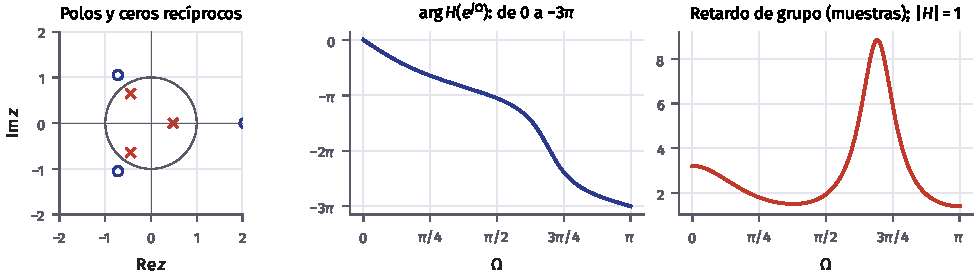
\includegraphics[width=0.95\linewidth]{paso_todo}
  \caption{Paso todo de orden 3 con $D(z)=1+0{,}4z^{-1}+0{,}18z^{-2}-0{,}3z^{-3}$: polos y ceros, fase y retardo de grupo.}\label{fig:paso-todo}
\end{figure}

\begin{propiedad}{Descomposición fase mínima por paso todo}{descomposicion}
  Todo sistema racional, causal y estable se puede escribir $H(z)=H_{\min}(z)\,H_{\text{PT}}(z)$, con $H_{\min}$ de fase mínima y $\abs{H_{\min}}=\abs H$.
\end{propiedad}

Basta reflejar hacia dentro cada cero $z_0$ con $\abs{z_0}>1$ y compensarlo con un paso todo de primer orden con el polo en $1/z_0^*$ y el cero en $z_0$. Por ejemplo,
\[
  \frac{1+3z^{-1}}{1-0{,}5z^{-1}}=\frac{3\,(1+\frac13z^{-1})}{1-0{,}5z^{-1}}\cdot\frac{\frac13+z^{-1}}{1+\frac13z^{-1}}.
\]
Como el paso todo siempre añade retardo, de aquí se deduce que el de fase mínima es el de menor retardo de grupo.

\subsection{Filtros en peine}

Sustituyendo $z$ por $z^L$ en un filtro $G(z)$ se obtiene un \emph{filtro en peine}:
\[
  H(z)=G(z^L),\qquad H(\e^{j\Omega})=G(\e^{j\Omega L}).
\]
La respuesta se comprime en un factor $L$ y se repite con periodo $2\pi/L$; en el tiempo, se intercalan $L-1$ ceros entre los coeficientes de $g[n]$. Con $G(z)=\frac12(1+z^{-1})$, que tiene un cero en $\Omega=\pi$, sale $H(z)=\frac12(1+z^{-L})$, con ceros en $\Omega=(2k+1)\pi/L$ (\cref{fig:peine}).

Para eliminar una frecuencia $f_0$ y todos sus armónicos, como el zumbido de la red eléctrica, se parte de una muesca en continua, $G(z)=\frac{1+a}{2}\frac{1-z^{-1}}{1-az^{-1}}$, y se toma $L=f_s/f_0$:
\[
  H(z)=\frac{1+a}{2}\,\frac{1-z^{-L}}{1-a\,z^{-L}}.
\]
Sus ceros son las $L$ raíces de la unidad, en $\Omega=2\pi k/L$, es decir, en $f=kf_0$; los polos están en los mismos ángulos con radio $a^{1/L}$. Cuanto más cerca de 1 está $a$, más estrechas son las muescas y más largo el transitorio. Es el filtro que proporciona \texttt{iircomb} en Matlab y en \texttt{scipy.signal}.

\begin{figure}[ht]
  \centering
  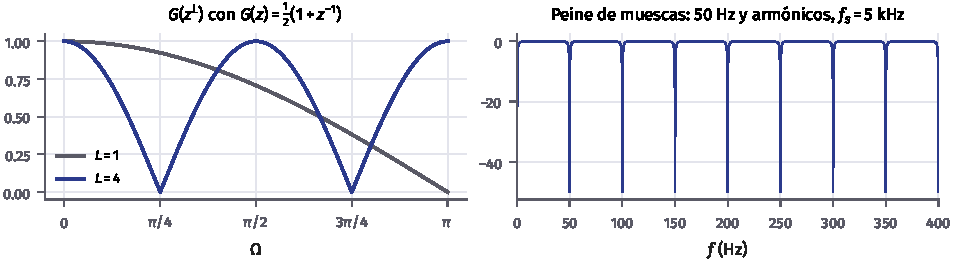
\includegraphics[width=0.95\linewidth]{peine}
  \caption{Peine FIR $\frac12(1+z^{-L})$ y peine de muescas para 50\,Hz y sus armónicos con $f_s=5$\,kHz.}\label{fig:peine}
\end{figure}

\begin{nota}[Erratas de versiones anteriores]
  El ejemplo antiguo de la red de 50\,Hz con $f_s=5$\,kHz calculaba $L=f_s/f_0=50$; es $L=5000/50=100$. El código asociado usaba además \texttt{iircomb(20,...)} y representaba la respuesta con $f_s=300$\,Hz, que no corresponden al enunciado.
\end{nota}

\begin{encodigo}
  Peine de muescas para 50\,Hz con $f_s=5$\,kHz y su respuesta en la componente útil (7\,Hz), en 50 y 150\,Hz y en 175\,Hz.
  \codigo{peine_50hz}
\end{encodigo}

\begin{flushright}\small\color{pdsgris}Ejercicios 16–18. \herramienta{server/T4\_05\_FIR\_Fase\_Cero.py}.\end{flushright}

% =====================================================================
\section*{Bibliografía}
\addcontentsline{toc}{section}{Bibliografía}

\begin{itemize}
  \item J.~G. Proakis y D.~G. Manolakis, \emph{Tratamiento digital de señales}, 4.ª ed. Pearson Prentice Hall, 2007. Capítulos 5 (fase mínima, paso todo) y 10 (diseño de filtros).
  \item A.~V. Oppenheim y R.~W. Schafer, \emph{Tratamiento de señales en tiempo discreto}, 3.ª ed. Pearson, 2011. Capítulos 5 (fase lineal, fase mínima y paso todo) y 7 (diseño de filtros).
  \item S.~K. Mitra, \emph{Procesamiento de señales digitales: un enfoque basado en computadora}, 3.ª ed. McGraw-Hill, 2007. Capítulos de diseño de filtros IIR y FIR; de ahí proceden los valores de la tabla de ventanas.
  \item F.~T. Ulaby y A.~E. Yagle, \emph{Signals and Systems: Theory and Applications}, 2.ª ed. Michigan Publishing Services, 2024. Capítulos de filtros. Descarga libre en\\ \url{https://services.publishing.umich.edu/Books/S/Signals-and-Systems}.
  \item V.~K. Ingle y J.~G. Proakis, \emph{Digital Signal Processing Using MATLAB}, 3.ª ed. Cengage Learning, 2012. Capítulos 7 y 8, con ejemplos en Matlab.
\end{itemize}

\end{document}
